\chapter{Foundations for inference}
\label{foundationsForInference}

Imagine the United States Center for Disease Control and Prevention (CDC) influencing policy makers in curbing the national obesity problem. The members of the CDC's Division of Nutrition, Physical Activity, and Obesity (DNPAO) "focus on policy and environmental strategies to make healthy eating and active living accessible and affordable for everyone." \footnote{\url{http://www.cdc.gov/obesity/}} Before they give policy suggestions, however, the DNPAO must first diagnose this problem of obesity in the United States. One metric that these scientists would consider could be a person's Body Mass Index, also known as BMI. A person's BMI has been a helpful tool to capture both a person's height and weight within one measurement and can be used as a measure of body fat. A high BMI can be an indicator for high body fat. In medicine, BMI can be used to categorize a person as "underweight," "overweight" or "obese." 

These policy makers can be interested in a couple of questions. What is the average population BMI for all adults in the United States? Instead of providing a single number, what is a plausible range values for the average BMI in the United States? Finally using the categorization of BMI values and ranges that the World Health Organization (WHO) provides, noting that it does not consider muscularity, is the average BMI in the United States considered an average healthy BMI? Below is a categorization of BMI values and ranges
\footnote{\url{http://apps.who.int/bmi/index.jsp?introPage=intro_3.html}}

\begin{center}
\begin{tabular}{|c|c|}
\hline 
Category & BMI range\tabularnewline
\hline 
\hline 
Underweight & $<18.50$\tabularnewline
\hline 
Normal (healthy weight) & 18.5-24.99\tabularnewline
\hline 
Overweight & $\geq 25$\tabularnewline
\hline 
Obese & $\geq30$\tabularnewline
\hline 
\end{tabular}
\end{center}

These questions encompass the broader idea of statistical inference in Chapter \ref{foundationsForInference}. Inference is a set of tools used to estimate properties or parameters about a population after observing a sample from this population. Inference also allows for different levels of quality or confidence of these parameter estimates. Once we have a parameter estimate, the average BMI in the United States for example, we can ask ourselves how confident we are that this estimate is representative of the greater population of the US. For example, a classic inferential question is, ``How sure are we that the estimated mean, $\bar{x}$, is near the population mean, $\mu$?'' Statistical inference includes asking these questions but also determining which estimates to use.

Chapter \ref {foundationsForInference} provides the groundwork for inference on a larger population from observing one sample, and later chapters will cover inference comparing two or more distinct populations. While the equations and details change depending on the setting, the foundations and general procedures for inference are the same throughout statistics. Understanding the foundation with point estimates in this chapter will provide familiarity for upcoming chapters. 

After looking at the data in Section \ref{brfssData} that the CDC could use in making these inferences, section \ref{variabilityInEstimates} will give us an introduction to point estimates, the sampling distribution that these estimates are drawn from and the variability of these estimates. Section \ref{confidenceIntervals} will give us tools to incorporate this variability. Rather than a single value, these policy makers can provide, instead, a confidence interval or a range of values that they believe are likely estimates. However with comparison, researchers might still want to compare point values against each other instead of ranges of values. Hypothesis testing in Section \ref{hypothesisTesting} allows the researchers to infer using point estimates while still encompassing the variability that the point estimates in section \ref{variabilityInEstimates} did not. The hypothesis testing framework gives us structure to do so and uses the same moving parts as a confidence interval. 

\section{BRFSS Data}
\label{brfssData}
The Behavioral Risk Factor Surveillance System (BRFSS) by the CDC was started in 1984 and is the world's largest on-going telephone health survey system. This survey is nationwide and aims to "monitor state-level prevalence of major behavioral risks among adults associated with premature morbidity and mortality." \footnote{\url{http://www.cdc.gov/brfss/about/about_brfss.htm}}  Topics like smoking, alcohol use, diet and exercise are included in this questionnaire. The annual survey data from 2000, \data{BRFSS}, includes records on 289 variables and could be used to estimate the average BMI of the US population. The variables that we are particularly interested in with calculating BMI are listed in Table  ~\ref{brfssBMIVariables}. 
\begin{comment} http://www.cdc.gov/brfss/annual_data/annual_2000.htm#information\end{comment}
\begin{table}[h]
\centering\small
\begin{tabular}{l p{65mm}}
\hline
{\bf variable} & {\bf description} \\
\hline
\var{sex} & Male or Female where 1 is Male and 2 is Female\\
\var{age} & In years \\
\var{height} & In feet and inches where, for example, 5' 5" is listed as 505 \\
\var{weight} & In pounds\\
\end{tabular}
\label{brfssBMIVariables}
\caption{Variables of interest and their descriptions for the \data{BRFSS} data set.}
\end{table}

The calculation of a BMI index from weight and height using both Metric and Imperial is \[BMI=\frac{\mathrm{weight_{kg}}}{\mathrm{height_{m}}^2}=\frac{\mathrm{weight_{lb}}}{\mathrm{height_{in}}^2}\cdot 703\]
where $\mathrm{weight_{kg}}$ and $\mathrm{height_{m}}$ is the weight and height measured in kilograms and meters while $\mathrm{weight_{lb}}$ and $\mathrm{height_{in}}$ is the weight and height in pounds and inches. 

Therefore by using the \data{BRFSS} data, we can use our sample of heights and weights to calculate BMI values for each observation. The \data{BRFSS} data comprises of 170,000 observations, and the CDC is hoping to infer the characteristics of adults in the United States, our target population. A target population is the group that the statistician is interested in and wants to draw conclusions about. 

We take a sample of 40,000 adults from the \data{BRFSS} data to use as our observed sample. We will refer to this random sample of 40,000 adults as \data{BRFSS BMI} from now on. Part of this dataset with the BMI calculation is shown in ~\ref{brfssBMIData}. 


% latex table generated in R 3.1.1 by xtable 1.7-4 package
% Sun Jul 19 13:57:10 2015
\begin{table}[ht]
\centering
\begin{tabular}{rrrrrr}
  \hline
 & sex & age & height & weight & bmi \\ 
  \hline
1 &   2 &  60 & 508 & 200 & 30.41 \\ 
  2 &   2 &  25 & 506 & 145 & 23.40 \\ 
  3 &   1 &  40 & 511 & 180 & 25.10 \\ 
  4 &   1 &  53 & 511 & 210 & 29.29 \\ 
  5 &   2 &  80 & 504 & 170 & 29.18 \\ 
  6 &   2 &  71 & 501 & 108 & 20.40 \\ 
   \hline
\end{tabular}
\caption{Six observations from the BRFSS BMI dataset} 
\label{brfssBMIData}
\end{table}


This simple random sample from \data{BRFSS} will be used to draw conclusions about the target population of US adults. This is the practice of statistical inference in the broadest sense. Let's explore the data with the tools from Chapter 1 in Figure~\ref{exploreBMI} before we estimate the average BMI in the US. 

\begin{figure}
\centering
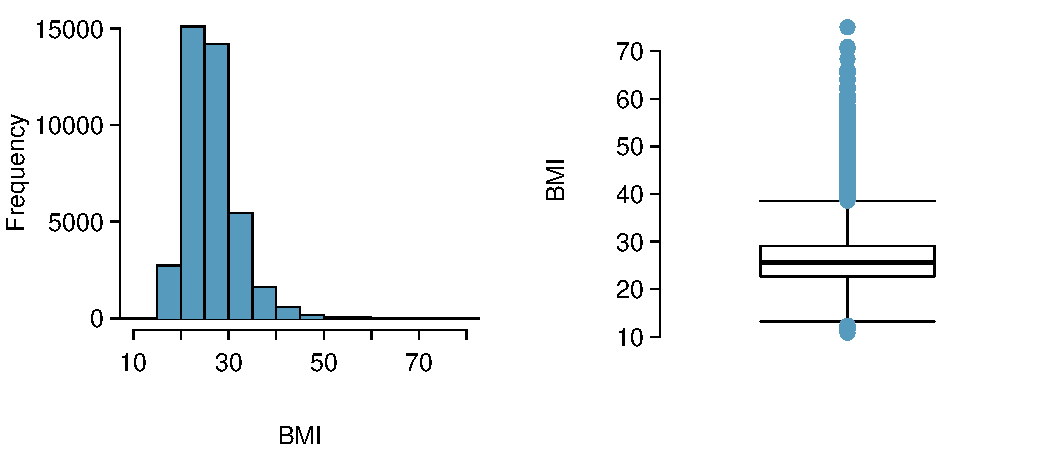
\includegraphics[width =  \textwidth]{ch_inference_foundations_oi_biostat/figures/brfssBMIsampHistograms/brfssBMIsampHistograms}
%hist(brfss.sample$bmi, main="Histogram of brfss.sample BMI", xlab="BMI")
%boxplot(brfss.sample$bmi, main = "Boxplot of brfss.sample BMI")
\caption{Histogram and boxplot of BMI for the \data{BRFSS BMI} data. The data is skewed right by both the histogram and the box plot. We can see from the box plot that it has many outliers}
\label{exploreBMI}
\end{figure}

The data from \data{BRFSS BMI} is special because in order to do statistical inference, the dataset needs to be representative of the population of interest. In this case, because the size of \data{BRFSS BMI} is so large and drawn randomly from \data{BRFSS}, we can assume that our data is representative and our estimates will be close to the population parameters.  Now that we have a general idea of what the data looks like, we can begin with statistical inference.

\section{Variability in estimates}
\label{variabilityInEstimates}

\index{point estimate|(}

If members at the CDC, after observing the sample of 40,000 BMI values, were asked to give their best guess for the average BMI in the US, what would it be? Here they would employ point estimation. A \term{point estimate} is a single value derived from sample data that serves as the "best guess" for that population parameter. Section ~\ref{variabilityInEstimates} will touch upon point estimates as well as the variability inherent in using this single number as the best guess. \footnote{While we focus on the the mean of BMIs in this chapter, questions regarding variation are often just as important in practice. For instance, potential action regarding obesity could change if the standard deviation of a person's BMI was 5 versus if it was 15.} 

\subsection{Point estimates}
\label{pointEstimates}

A likely choice to estimate the \term{population mean} from our sample is to simply take the \term{sample mean}. That is, use the average BMI of all 40,000 survey respondents in our sample as our estimate for the average BMI among US adults. 

For notation, use $\mathrm{bmi}_1, \mathrm{bmi}_2, \ldots, \mathrm{bmi}_{40,000}$  to represent the BMI for each survey respondent in our sample \data{BRFSS BMI}. The sample mean for BMI using our 40,000 observations is 
\begin{eqnarray*}
\bar{\mathrm{bmi}} = \frac{30.40 + 23.40 + 25.10 + \dots}{40,000} = 26.356
\end{eqnarray*}
\index{point estimate!single mean|(}
and is the \term{point estimate} of the population mean\footnote{If we were interested in the values of another variable, \var{weight} denoted $w_1,\ldots w_{40,000}$ instead, we would denote the sample mean as $\bar{w}$}. 

Suppose from the original respondents in \data{BRFSS}, we take a new sample of 40,000 people and recompute the mean; we will probably not get the same answer that we got using the \data{BRFSS BMI} data set. Estimates generally vary from one sample to another even with the same sample size, and low \term{sampling variation} can suggest our estimate may be close, but not exactly equal to the parameter. A larger sample size can ensure a closer estimate to the population parameter. In 2000, the US population was 282.2 million, \footnote{\url{http://www.census.gov/prod/2002pubs/c2kprof00-us.pdf}} 7,000 times our sample size of 40,000. 

What about generating point estimates of other \term{population parameters}, such as the population median or population standard deviation? We can estimate parameters based on sample statistics. For example, we estimate the population standard deviation for BMI using the sample standard deviation, and the population median using the sample median. Table ~\ref{BMIEstimates} provides the point estimates to other population parameters relating to BMI.

% latex table generated in R 3.1.1 by xtable 1.7-4 package
% Sun Jul 19 20:25:13 2015
\begin{table}[ht]
\centering
\begin{tabular}{lr}
  \hline
BMI & estimates \\ 
  \hline
mean & 26.356 \\ 
  median & 25.620 \\ 
  std. dev. & 5.288 \\ 
   \hline
\end{tabular}
\caption{Point estimates for the \var{bmi} variable} 
\label{BMIEstimates}
\end{table}

\begin{exercise} \label{pointEstimateOfDesiredWeights}
Suppose we want to estimate the average age for men and women in the US. If $\bar{\mathrm{age}}_{\mathrm{women}} = 47.35 $ years and $\bar{\mathrm{age}} _ {\mathrm{men}} = 45.67 $ years, what would be a good point estimate for the population age difference? \footnote{We could take the difference of the two sample means: $47.35 - 45.67 =  1.69$. Women are on average older than men by 1.69 years.}
\end{exercise}
%men = brfss.sample[which(brfss.sample$sex == 1),]
%women = brfss.sample[which(brfss.sample$sex == 2),]
%mean(women$age) - mean(men$age)

\begin{exercise}
If you had to provide a point estimate of the population IQR for the BMI of participants, how might you make such an estimate using a sample?\footnote{To obtain a point estimate of the IQR for the population, we could take the IQR of the sample.}

\index{point estimate!single mean|)}

\end{exercise}

The sample mean calculated from this \data{BRFSS BMI} sample of 40,000 will likely be different from the sample mean of a different set of 40,000 respondents from \data{BRFSS} data. Using $R$, we take another random sample from the \data{BRFSS} data of 40,000 and see that that the new sample mean for the BMI is 26.344. We note that estimates will differ across samples through sampling variation but the accuracy of the point estimate will get improve once more data becomes available and sample sizes increase.

Consider a running mean from the \data{BRFSS BMI} data to explore increases in sample size. A \term{running mean} is a sequence of means, where each mean uses one more observation in its calculation than the mean directly before it in the sequence. In this case, the second mean is the average of the first two observations, $\mathrm{bmi}_1, \mathrm{bmi}_2$. The third number in the running mean sequence is the average of $\mathrm{bmi}_1, \mathrm{bmi}_2,$ and $\mathrm{bmi}_3$. 

The running mean for \data{bmi} in the \data{BRFSS BMI} dataset is shown in Figure~\ref{BMIRunningMean}. We look at a running mean of 300 and 5000 observations. We note that as more values get included, the running mean converges closer to the sample mean of 26.36. Similarly if the sample size increases from 40,000 to 100,000, the sample mean from 100,000 observations will be closer to the average US population BMI than the sample mean of 40,000 observations. 

\begin{figure}
   \centering
   \includegraphics[width=\textwidth]{ch_inference_foundations_oi_biostat/figures/brfssBMIRunningMean/brfssBMIRunningMean}
   \caption{The running means from the \var{BRFSS BMI} sample of 40,000 observations. The mean stabilizes and approaches the mean of the entire sample $\bar{x} = 26.36$ as the number of observations increases}
      \label{BMIRunningMean}
\end{figure}

Sampling variation, however, is across samples of the same size. Figure ~\ref{runningSamplingVariation} displays the running means of two samples and of 20 samples. We see at each observation that the sample mean is not the same. There exists some sampling variation. Even more interesting, the variation decreases as the number of observations increases. We will explore this concept more in Section ~\ref{accuracyAndPrecision}. 

\begin{figure}
   \centering
   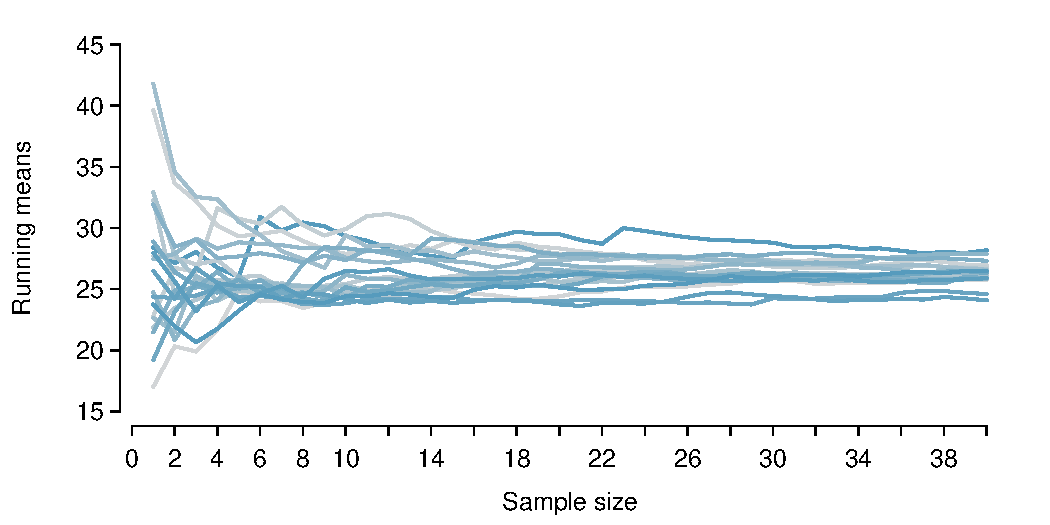
\includegraphics[width=\textwidth]{ch_inference_foundations_oi_biostat/figures/brfssBMISampVar/brfssBMISampVar20}
   \caption{Many running means from different samples of 40,000 observations from \data{BRFSS}. The sampling variation decreases as the number of observations gets larger.}
	\label{runningSamplingVariation}
\end{figure}



\subsection{Accuracy and Precision of Point Estimates}
\label{accuracyAndPrecision}

Accuracy and precision have colloquially become interchangeable. In science, however, they both have very distinct meanings. Accuracy is a characteristic of how close the measurements are to their true value. Precision is the characteristic of how close the measurements are to themselves. 

Within inference and point estimates, the sample mean is always accurate. The sample mean does not contain any systematic error. The sample mean is only not equal to the population mean because of random sampling error. While the sample mean may not always be equal to the population mean, in expectation, the sample mean and population parameter are equivalent. We observe the accuracy of the sample mean in practice with 20 running means from Figure ~\ref{runningSamplingVariation}. The center of these running means is, in expectation, the population average BMI. 

While the sample mean is consistently accurate, it may not always be precise. As the sample size, n, increases, the randomness in the sample mean decreases. We look to sampling variation at different sample sizes as evidence. Figure ~\ref{sampleMeanPrecision} shows two histograms of sample means. The left histogram has sample means with a sample size of 5 and the right has a sample size of 50. All of these samples are randomly drawn from the \data{BRFSS} data, the sample mean calculated and plotted as an observation on the histogram. The histogram with $n=50$ has noticeably smaller variance than the histogram with $n=5$. The histogram with $n=5$ is also slightly skewed. As such, with larger sample sizes, the sample variation decreases, making the sample mean more precise across samples. We look to Section ~\ref{seOfTheMean} to quantify and measure sampling variation as more data becomes available. 

\begin{figure}
   \centering
   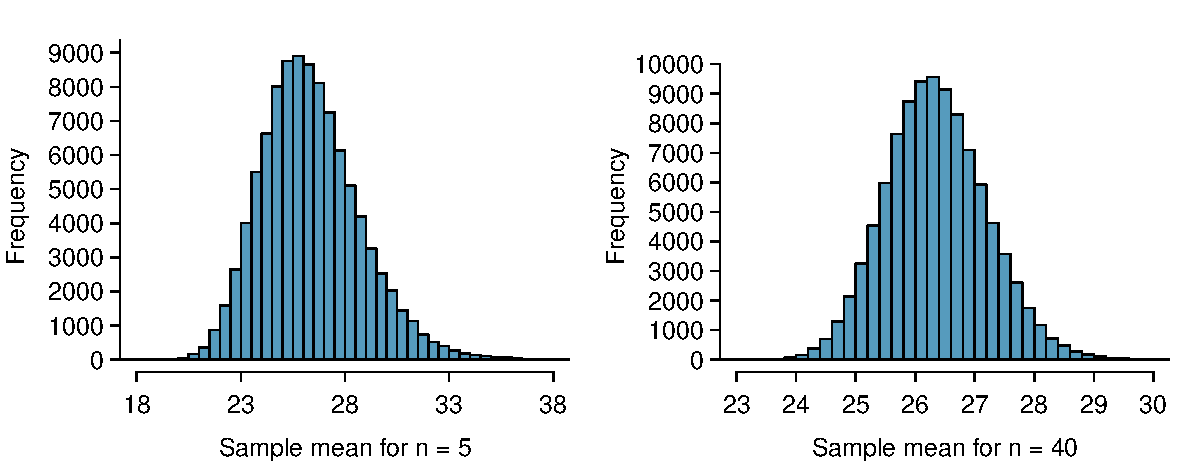
\includegraphics[width=\textwidth]{ch_inference_foundations_oi_biostat/figures/brfssBMISampleMeanPrecision/brfssBMISampleMeanPrecision}
   \caption{Sample means of size $n=5$ and $n=50$.}
   \label{sampleMeanPrecision}
\end{figure}
 
\subsection{Sampling Distribution and the Standard Error of the Mean}
\label{seOfTheMean}

From the random sample represented in \data{BRFSS BMI}, we estimated the average BMI of an adult in the United States to be 26.356. Suppose we take another random sample of 40,000 individuals and take its mean. In Section ~\ref{pointEstimates}, we then get 26.359. Suppose we took another (26.350) and another (26.349), and continue to do this many many times -- which we can do only because we have access to the larger \data{BRFSS} dataset. \footnote{The sampling distribution depends on the underlying distribution of the target population. In this case, while \data{BRFSS} is not quite the target population of all US adults, it is large enough illustrate the concept of sampling distribution and acts as a representative substitute to the US population. If we had complete data from the target population, there would be no need to take a sample mean measurement. In practice, we generally aren't even capable of taking another sample of 40,000 from \data{BRFSS}!} We can then build up a \term{sampling distribution} for the sample mean when the sample size is 40,000, shown in Figure~\ref{brfssBMISamplingDistribution}.

\begin{termBox}{\tBoxTitle{Sampling distribution}
The \term{sampling distribution} of a point estimate represents the distribution of the point estimate based on samples of a fixed size from a certain population. There is a unique sampling distribution that exists that is inherent to the point estimator you are measuring. Every time that you are calculating your point estimate from a particular sample of said size, your point estimate s one sample from the sampling distribution. Understanding the concept of a sampling distribution is central to understanding statistical inference.}
\end{termBox}


\begin{figure}
   \centering
   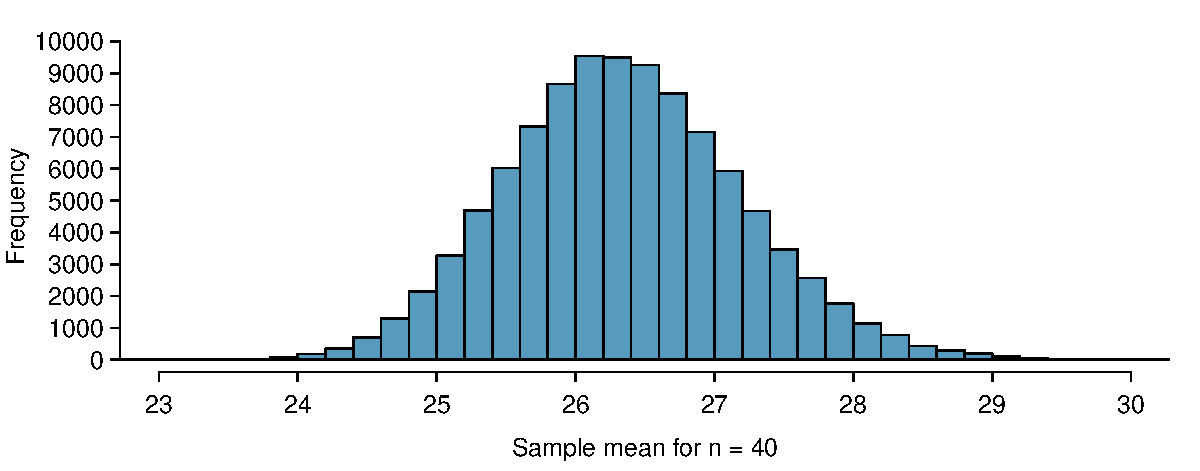
\includegraphics[width=0.85\textwidth]{ch_inference_foundations_oi_biostat/figures/brfssBMISamplingDistribution/brfssBMISamplingDistribution}
   \caption{A histogram of 100,000 sample means for BMI, where the samples are of size $n=40,000$. }
      \label{brfssBMISamplingDistribution}
\end{figure}

Figure~\ref{brfssBMISamplingDistribution} is an approximation of the sampling distribution. To truly get the sampling distribution, one would need to sample every possible unique combination of 40,000 respondents from the entire US adult population (and not just the \data{BRFSS} data set). However we note that just as the running mean becomes a better approximation of the population average as more data becomes available, the approximation of the sampling distribution also resembles more closely the sampling distribution as we take more and more samples. We note again that precision increases significantly as the sample size $n=40,000$ with the sample means of $n=40,000$ ranging from 26.25 to 26.45, a much smaller range than for $n=5$ or $n=50$ in Figure ~\ref{sampleMeanPrecision}. We can create an approximation of the sampling distribution of the sampling mean with the following pseudocode \footnote{Refer to the appendix for R code}: 

\begin{verbatim}
(1) Have a place to store all the sample means that we will calculate
(2) Take a sample from the BRFSS dataset of 40,000
(3) Calculate the sample mean from this specific sample and store it in (1)
(4) Repeat (2) and (3) many many times 
(5) Plot all the sample means you have stored in (1) as a histogram
\end{verbatim}
  
The sampling distribution, in this case, is likely to be unimodal and approximately symmetric. The sampling distribution is also centered exactly at the \data{BRFSS} population mean: $\mu=26.351$. Intuitively, this makes sense. The sample means should tend to ``fall around'' the mean that we are drawing from.

By the sampling distribution, we also see that the point estimator will have some variability. We see the concept of sampling distribution introduced in Section ~\ref{accuracyAndPrecision} and note that the precision increases as the sample size gets larger. Point estimates, however, still vary sample by sample. There needs to be some metric to quantify the variability of the sample mean around the population mean.

\begin{tipBox}{\tipBoxTitle{More data means less variability}
In sampling, the larger the sample size the better. The precision of the sample mean increases as you observe more data in your sample.}
\end{tipBox}

Standard deviation is the most obvious method to quantify variability. We use the standard deviation of the sampling distribution denoted  $\sigma_{\bar{x}}$ or $s$ in some contexts to measure sampling variation of the sample mean. \footnote{Caution: The standard deviation of the sample mean is not equivalent to the estimate for the standard deviation of the population. Those are measuring two separate quantities.}

Just as with the definition of standard deviation in \textbf{Chapter 1}, the standard deviation of the sample mean, tells us how far the typical estimate is away from the actual population mean. It also is a very good metric for the typical \term{error} of the point estimate, and for this reason we usually call this version of standard deviation the \term{standard error (SE)} \index{SE}\marginpar[\raggedright\vspace{-4mm} $SE$\\\footnotesize standard\\error]{\raggedright\vspace{-4mm} $SE$\\\footnotesize standard\\error} of the estimate. \footnote{In general, standard error is the standard deviation of samples and estimates whereas we use the term standard deviation for populations or distributions. Look AT \textbf{SOME REFERENCE} for a clearer distinction of standard error versus standard deviation.} 

\begin{termBox}{\tBoxTitle{Standard error of an estimate}
The standard deviation associated with an estimate is called the \emph{standard error}. It describes the typical error or uncertainty associated with the estimate.}
\end{termBox}

\begin{exercise}
(a) Would you rather use a small sample or a large sample when estimating a parameter? Why? (b) Using your reasoning from (a), would you expect a point estimate based on a small sample to have smaller or larger standard error than a point estimate based on a larger sample?\footnote{(a) Consider two random samples: one of size 10 and one of size 1000. Individual observations in the small sample are highly influential on the estimate while in larger samples these individual observations would more often average each other out. The larger sample would tend to provide a more accurate estimate. (b) If we think an estimate is better, we probably mean it typically has less error. Based on (a), our intuition suggests that a larger sample size corresponds to a smaller standard error.}
\end{exercise}

The standard error could be calculated if statisticians knew the sampling distribution. It would simply be the standard deviation of that sampling distribution. However when considering the case of the point estimate $\bar{x}$, there is one problem: most often, scientists only observe one sample, and there is no obvious way to estimate its standard error from a single sample. Computation methods and statistical theory, instead, provide helpful tools to address this issue. 

Instead of only observing one sample from \data{BRFSS}, imagine if we could repeatedly sample from \data{BRFSS} as with creating the approximation to the sampling distribution. After many iterations, the standard deviation of the sample means becomes a fairly reasonable estimate of the standard error of the sample mean. In pseudocode: 
\begin{verbatim}
(1) Have a place to store all the sample means that we will calculate
(2) Take a sample from the BRFSS dataset of 40,000
(3) Calculate the sample mean from this specific sample and store it in (1)
(4) Repeat (2) and (3) many many times 
(5) Calculate the standard deviation of the values in (1). This is an 
	estimation of your standard error
\end{verbatim}

Again what we are doing in $R$ is creating an approximate sampling distribution and then using the standard deviation from this approximation to be our estimate for the standard error. We do this with the following code:\footnote{This computing experience samples without replacement to simulate experimenting in the real world. Theory states however that individual BMI values need to be independent. A reliable method to ensure sample observations are independent is to guarantee that the sample from the population is a simple random sample with a size that is less than 10\% of the population. This 10\% rule, remember, is used as a rule of thumb. By sampling without replacement within a finite population, we will see that \var{sd(sample.means)} is not exactly the theoretical standard error but quite close.}
\begin{verbatim}
> sample.means<-matrix(data=NA,nrow=1000, ncol=1) #to store the sample means
> for(i in 1:1000){
+   sample<-sample(x=brfss.df$bmi, size=40000, replace=FALSE)
+   sample.means[i]<-mean(sample)
+ }
> sd(sample.means)
[1] 0.02359317 
\end{verbatim}

%While we do not have the exact sampling distribution, we do have the ability to calculate an approximate standard error. 

This method, however, has one main issue. Practitioners rarely are able to repeatedly sample from their larger population. Instead the standard error of the sample mean can be calculated through the following equation: 

\begin{termBox}{\tBoxTitle{Computing SE for the sample mean}
Given $n$ independent observations from a population with standard deviation $\sigma$, the standard error of the sample mean is equal to \vspace{-1mm}
\begin{eqnarray}
SE_{\text{ sample mean}} = \frac{\sigma}{\sqrt{n}}
\label{seOfXBar}
\end{eqnarray}\vspace{-3mm}%

A reliable method to ensure sample observations are independent is to guarantee that the sample you have from the population is a simple random sample with a size that is less than 10\% of the population.\index{standard error!single mean}
}
\end{termBox}

There is one subtle issue of Equation~(\ref{seOfXBar}) that you might have realized: the population standard deviation is typically unknown. To resolve this problem, we can use the point estimate of the standard deviation from the sample. This estimate tends to be sufficiently good when the sample size is at least 30 and the population distribution is not strongly skewed. Thus, we often just use the sample standard deviation denoted $s$ instead of~$\sigma$ for the population standard deviation. When the sample size is smaller than 30, we will need to use a method to account for extra uncertainty in the standard error. If the skew condition is not met, a larger sample is needed to compensate for the extra skew. These topics are further discussed in Section~\ref{cltSection}. 

With the \data{BRFSS BMI} sample of 40,000, the standard error of the sample mean is calculated as

\begin{eqnarray*}
SE_{\bar{x}} = \frac{s}{\sqrt{n}} = \frac{5.288}{\sqrt{40000}} =  0.026
\end{eqnarray*}
where $s$ is the standard deviation of the sample and $n$ is the number of observations in the sample. We see that the standard error calculated $(0.026)$ is similar to the empirical standard deviation of the sampling distribution $(0.024)$. 

\begin{exercise}
In another sample of 40,000 US adults, the standard deviation of BMI is $s_y = 5.34$. Because the sample is a simple random sample and consists of less than 10\% of the United States population, the observations are independent. (a)~What is the standard error of the sample mean, $\bar{y}=26.36$? (b)~Would you be surprised if someone told you the average BMI of all US adults was actually 30? What about 26? \footnote{(a) Use Equation~(\ref{seOfXBar}) with the sample standard deviation to compute the standard error: $SE_{\bar{y}} = 5.34/\sqrt{40000} =  0.0267$. (b) It would be surprising if the true average BMI was 30. A BMI of 30 is many standard deviations away from the sample mean of 26.36. In other words, a BMI of 30 seems implausible given that our sample mean (26.36) is far from the "true mean" using the standard error of 0.0267 to identify what is close and what is not close. Even a BMI of 26 in this situation would be surprising given that is it more than one standard deviation away from the sample mean (standard error of 0.0267).}
\end{exercise}
%include code


\begin{exercise}
(a) Would you be more trusting of a sample that has 100 observations or 400 observations? (b) We want to show mathematically that our estimate tends to be better when the sample size is larger. If the standard deviation of the individual observations is 10, what is our estimate of the standard error when the sample size is 100? What about when it is 400? (c) Explain how your answer to (b) mathematically justifies your intuition in part~(a).\footnote{(a) Look back to Section ~\ref{accuracyAndPrecision} on accuracy and precision. Extra observations are usually helpful in understanding the population, so a point estimate with 400 observations seems more trustworthy. (b) The standard error when the sample size is 100 is given by $SE_{100} = 10/\sqrt{100} = 1$. For 400: $SE_{400} = 10/\sqrt{400} = 0.5$. The larger sample has a smaller standard error. (c) The standard error of the sample with 400 observations is lower than that of the sample with 100 observations. The standard error describes the typical error, and since it is lower for the larger sample, this mathematically shows the estimate from the larger sample tends to be better -- though it does not guarantee that every large sample will provide a better estimate than a particular small sample.}
\end{exercise}

\subsection{Basic properties of point estimates}

We achieved three goals in this section. First, we determined that point estimates from a sample may be used to estimate population parameters. We also determined that these point estimates are not exact, and there exists some sampling variation. The sample mean is an example of a point estimate that is always accurate but not necessarily always precise. The precision of a point estimate can be represented through sampling variation and visualized through a sampling distribution, and the point estimate that we observe is a single observation in the estimate's entire sampling distribution. Lastly, we quantified this sampling variation and the uncertainty of the sample mean using what we call the standard error. The standard error of the sample mean can be mathematically represented in Equation~\eqref{seOfXBar} or through computation with $R$. While we could also quantify the standard error for other estimates -- such as the median, standard deviation, or any other number of statistics -- we will postpone these extensions until later chapters and courses.

\index{point estimate)}

%__________________
\section{Confidence intervals}
\label{confidenceIntervals}

\index{confidence interval|(}

A point estimate, we saw in Section~\ref{pointEstimates} provides a single plausible value for a parameter. However, a point estimate is rarely perfect and exact; usually there is some error in the estimate. We know that there exists sampling variation but a single point estimate does not convey how large this sampling variation is without including the point estimate's standard error. Instead of supplying just a point estimate, the next logical step would be to provide a plausible \emph{range of values} to estimate the true value of the parameter.

In this section and in Section~\ref{hypothesisTesting}, we will emphasize the special case where the point estimate is a sample mean and the parameter that we are interested in is the population mean. In Section~\ref{aFrameworkForInference}, we generalize these methods for a variety of point estimates and population parameters that we will encounter in Chapter~\ref{inferenceForNumericalData} and beyond.

\subsection{Capturing the population parameter}

A plausible range of values for the population parameter is called a \term{confidence interval}. The width of an interval provides a gauge of how large the sampling variation is. For the same confidence level, the larger the interval indicates the larger sampling variation and standard error.

Using only a point estimate is like fishing in a murky lake with a spear, and using a confidence interval is like fishing in the same lake with a net. We can throw a spear where we see fish, but we will probably miss. On the other hand, if we toss a net in that area, we have a good chance of catching the fish.

If we report a point estimate, we probably will not hit the exact population parameter. There is likely to be some error associated with this estimate. On the other hand, if we report a range of plausible values -- a confidence interval -- we have a good shot at capturing the parameter within our range. As with fishing, the goal of the confidence interval is to include the population parameter within it. 

\begin{exercise}
If we want to be very certain we capture the population parameter, should we use a wider interval or a smaller interval?\footnote{If we want to be more certain we will capture the fish, we might use a wider net. Likewise, we use a wider confidence interval if we want to be more certain that we capture the parameter. The more values we include in our range, the more likely it is that this range contains the true value since the interval contains simply \emph{more} values. However just capturing the parameter with the widest interval is not always the best when constructing a confidence interval. We can always capture the parameter with an interval going from $-\infty$ to $+\infty$ but does range does not increase our understanding of the population parameter.}
\end{exercise}
\begin{exercise}
Suppose we have a confidence interval that is 10 units wide and that we are 50\% confident that the range encompasses the population parameter. If we had another interval that was instead 5 units wide centered at the same value as our original interval, are we now more or less confident than 50\% that the range will include the population parameter? \footnote{We are less confident than 50\% that the smaller interval includes the population parameter simply because it is smaller and contains fewer values. Using a smaller net, we are less confident that we have captured the true value.}
\end{exercise}

\subsection{Confidence levels}

The size of our fishing net depends on how confident we want to be in catching a fish. Similarly, the size or width of our confidence intervals depends on how confident we want to be in estimating the true value of the parameter in question. Before we even jump into the calculation of the confidence interval itself, let's first understand what it means to be "confident." 

Before scientists embark on most inference processes, they first much choose a confidence level. For a confidence interval, the confidence level is a percent that affects how wide the interval you calculate is. Confidence levels, in general, are associated with a level of uncertainty and how much you are allowing your test to commit a Type I Error or a false positive. Section~\ref{DecisionErrors} goes into more depth on Type 1 and Type 2 Errors. 

For example if you wanted to say that we are 75\% confident that the population mean BMI is between two values, 75\% would be our measure of uncertainty and 25\% would be the probability of committing a Type 1 Error. In the context of confidence intervals, there is a 25\% chance that the confidence interval does not include the population parameter when in fact, it should. The Type I error is also known as $\alpha$.  

\begin{example}{Consider extreme confidence levels. What are the implications of a 100\% confidence level confidence interval? How about a 0.001\% confidence level?} \label{extremeConfidenceLevels}
A 100\% confidence level is equivalent to $\alpha = 0\%$. The confidence interval we create will \emph{always} capture the population parameter. Therefore in order to guarantee this, the confidence interval will be $[-\infty, \infty]$ . Consider a confidence level of 0.001\%. This extremely low confidence level results in a very high Type 1 Error. In many cases when building a 0.001\% confidence interval, the confidence interval will not capture the population parameter. Therefore we can foresee this interval being extremely narrow. 
\end{example}

Statisticians generally use a confidence level of 95\% per tradition but Section ~\ref{significanceLevel} demonstrates that any confidence level is allowed given varying inference goals in mind. But what does "95\% confident" truly mean? Suppose we took many samples and built a confidence interval based on each sample. Then to be 95\% confident, we would see approximately 95\% of those intervals would contain the actual mean, the population parameter, $\mu$. In this case, if we took 100 independent samples and built 100 confidence intervals, 95 of these confidence intervals would contain the average US BMI and 5 of these would not.

Figure~\ref{95PercentConfidenceInterval} shows this process with 25 samples, where 24 of the resulting confidence intervals contain the average BMI for the population and one does not.

\begin{figure}[hht]
   \centering
   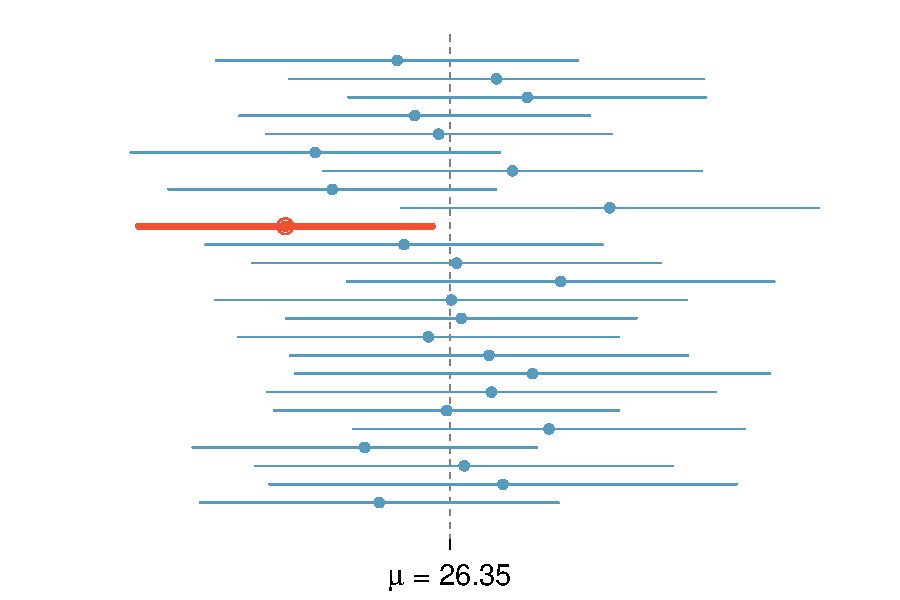
\includegraphics[width=0.75\textwidth]{ch_inference_foundations_oi_biostat/figures/95PercentConfidenceInterval/95PercentConfidenceInterval}
   \caption{Twenty-five samples of size $n=100$ were taken from the \data{BRFSS} data set. For each sample, a confidence interval was created to try to capture the average BMI for the population. Only~1 of these~25 intervals did not capture the true mean.}
   \label{95PercentConfidenceInterval}
\end{figure}

\subsection{Confidence intervals through computation}

Figure~\ref{95PercentConfidenceInterval} should give you inspiration on how to achieve an estimate of a 95\% confidence interval through computation. Our goal, again, is to find a range of values that hopefully contains the population parameter. If we have the ability to independently resample from our population, the natural method to estimate a confidence interval is through the sampling distribution like in Figure~\ref{brfssBMISamplingDistribution}. We observed there that the mean of the sampling distribution was extremely close to the mean of the population we were sampling from. Thus a reasonable estimation for a 95\% confidence interval would be to take the middle 95\% of the sampling distribution. Below we have pseudocode that implements this procedure \footnote{This highly resembles the pseudocode for approximating a sampling distribution from Section ~\ref{seOfTheMean}}
\begin{verbatim}
(1) Have a place to store all the sample means that we will calculate
(2) Take a sample from the BRFSS dataset of 40,000
(3) Calculate the sample mean from this specific sample and store it in (1)
(4) Repeat (2) and (3) many many times 
(5) Use the middle 95% of values as the 95% confidence interval. 
\end{verbatim}

We can build off the method of approximation the sampling distribution to compute a 95\% confidence interval. Instead of plotting the values of the sample means (stored as \var{sample.means} within the $R$ code) to create the sampling distribution, we can find the values to get the middle 95\% of sample means.  

The confidence interval itself is the BMI value  $c_1$ such that 2.5\% of the \var{sample.mean} values is below $c_1$ and another BMI value $c_2$ such that 2.5\% of the distribution values is greater than $c_2$. In order to find these values, recall from the distributions unit ~\ref{distributions} that we need to use the \var{quantile()} function in $R$. Particularly using \var{sample.means} as the vector that that stores the sample means. 
\begin{verbatim}
confidence.interval<-quantile(x=sample.means,c(0.025,0.975))
> confidence.interval
    2.5%    97.5% 
26.30493 26.39697 
\end{verbatim}
We see that the interval (26.30,26.40) is an estimation for a 95\% confidence interval using the sampling distribution of sample means. Therefore we can say that we are 95\% confident that the population mean BMI is between 26.30 and 26.40. Similarly we can also say that after calculating many confidence intervals from many different observed samples, 95\% of all the confidence intervals that we calculated will contain the population mean. 

\begin{exercise}
Say we were interested in creating a 90\% confidence interval and a 50\% confidence interval. (a) how do you think the widths of the confidence intervals would compare? (b) How would we use the \var{quantile()} function to find the 90\% and 50\% confidence intervals from using the array \var{sample.means}?
 \footnote{(a) We would expect the 50\% confidence interval would have the smaller width. In general the more confident we are, the larger the confidence interval width will be.(b) Remember we want the middle percent of observed sample means. Therefore for the 90\% confidence interval using \var{sample.means} again to store the sample means, the $R$ code would be \var{quantile(x=sample.means,c(0.05,0.95))}. For a 50\% confidence interval, the code would be \var{quantile(x=sample.means,c(0.25,0.75))}}
\end{exercise}

\subsection{Calculating an approximate 95\% confidence interval}
Computing the confidence interval from resampling is straightforward and serves as a great estimate for any confidence interval for the population. However we ask ourselves, is this realistic beyond simulation? In general do we have the ability to resample the US population independently 100,000 times? Generally no. Most times we cannot observe 100,000 sample means of BMI values let alone 100,000 complete samples from the US population. More often than not, researchers only view 1 sample and thus calculate only 1 sample mean. How then do we calculate a confidence level from only observing one sample mean? 

We see from the computation in Section ~\ref{seOfTheMean} and Figure ~\ref{brfssBMISamplingDistribution} that the sampling distribution is centered around the population mean and that a confidence interval is derived from that sampling distribution. Therefore it becomes intuitive to build the confidence interval around the observed sample mean  as the point estimate is the most plausible value for the population parameter. The width of the interval should encompass the confidence level as well as the uncertainty associated with the point estimate. The standard error becomes a natural measurement of uncertainty for building the interval.  

Roughly 95\% of the time, the estimate that is observed from resampling will be within approximately 2 standard errors\footnote{1.96 to be more precise if the sampling distribution resembles a Normal Distribution. Details coming up in Section ~\ref{sampdistmean}} of the population parameter. Therefore we can create a 95\% confidence interval that is 2 standard errors from the point estimate on either side of the sample mean. We then can be roughly \term{95\% confident} that we have captured the population parameter with the confidence interval calculated by Equation ~\ref{95PercentConfidenceIntervalFormula} from the sample that we observe:
\begin{eqnarray}
\text{point estimate}\ \pm\ 2 \times SE \footnote{95\% confidence corresponds closer to 1.96 standard errors away} 
\label{95PercentConfidenceIntervalFormula}
\end{eqnarray}
Using the BMI sample from ~\ref{seOfTheMean} with an observed sample mean of 26.36 and sample standard deviation of 5.29, we calculate  the 95\% confidence interval. 
\begin{align*}
\text{point estimate}\ &\pm\ 2 \times SE\\
26.36 &\pm 2\times \frac{5.29}{\sqrt{40000}}\\
26.36 &\pm  0.053\\
(26.31 &, 26.41)
\end{align*}
While not exact, we see that the confidence interval simulated through $R$  achieves a very similar confidence interval as the one above through calculation. The difference is due to randomness within the samples since both the point estimate and the standard error vary among samples.
\begin{exercise}
In Figure~\ref{95PercentConfidenceInterval}, one interval does not contain a BMI value of 26.36. Does this imply that the average population BMI cannot be 26.36? \footnote{Just as some observations occur more than 2 standard deviations from the mean, some point estimates will be more than 2 standard errors from the parameter. A confidence interval only provides a plausible range of values for a parameter. While we might say other values are implausible based on the data, this does not mean they are absolutely impossible.}
\end{exercise}

We forewarn that "about 95\% of observations are within 2 standard deviations of the mean" is only approximately true. This rule of thumb holds very well for the normal distribution. As we will soon see in Section ~\ref{cltSection}, the sample mean tends to be normally distributed when the sample size is sufficiently large. 

\begin{example}{We are curious about how the average heights of men and women differ and create 95\% confidence intervals for the average male height and the average female height. The \data{BRFSS BMI} data can be divided using the \var{sex} variable. Among the 40,000 individuals within the \data{BRFSS BMI}, there are 16,843 men and 23,157 women. The average male height is 70.22 inches and the average female height is 64.38. The sample standard deviations for males and females  are 3.00 and 2.80 respectively. What are the 95\% confidence intervals for the average male and female height in the US? }\label{CIforGenderHeight}
We calculate both 95\% confidence intervals using the formula \[\text{point estimate}\ \pm\ 2 \times SE\] using the information given above: 
\begin{align*}
\text{men: point estimate}\ &\pm\ 2 \times SE\\
70.22 &\pm 2\times \frac{3.00}{\sqrt{16843}}\\
70.22 &\pm  0.05 \\
(70.17 &, 70.27)
\end{align*}
\begin{align*}
\text{women: point estimate}\ &\pm\ 2 \times SE\\
64.38 &\pm 2\times \frac{2.80}{\sqrt{23157}}\\
64.38 &\pm  0.04\\
(64.34 &, 64.42)
\end{align*}
The confidence intervals for average height by gender are different. With different centers and different widths, the underlying distributions for male and female heights are different. \end{example}

The creation of the 95\% confidence interval depends on the center and the standard error. In Section ~\ref{changingTheConfidenceLevelSection}, we will see how the multiplier changes beyond 2 standard deviations as confidence levels change. 

\begin{exercise} \label{95CIExerciseForBRFSSAge}
The sample data \data{BRFSS BMI} suggest the average adult's age is about 46.64 years with a standard error of 0.09 years (estimated using the sample standard deviation, 17.35). What is an approximate 95\% confidence interval for the average age of US adults?\footnote{Again apply Equation~(\ref{95PercentConfidenceIntervalFormula}): $46.64 \ \pm \ 2\times 0.09 \rightarrow (46.46, 46.82)$. We interpret this interval as follows: We are about 95\% confident the average age of US adults was between 46.46 and 46.82 years. Looking at the entire dataset \data{BRFSS} that represents the US population more closely (normally we do not have this luxury!) we see that the average age is 46.72 which is indeed within our confidence interval.}
\end{exercise}

\subsection{The sample size for a sampling distribution}
\label{sampdistmean}

In Section~\ref{seOfTheMean}, we introduced a sampling distribution for $\bar{x}$, the average BMI value for samples of size 5 and 50. We examined this distribution earlier in Figure~\ref{brfssBMISamplingDistribution}. We see with larger sample sizes like $n=40,000$, the sampling variation decreases significantly than if $n=5$ or $n=50$. In Figure ~\ref{sampleMeanPrecision}, the sampling distribution for $n=5$ was slightly skewed but the sampling distribution for $n=50$ looks more symmetric. We show in Figure \~ref{sampDistNormal} a histogram of the sample means for 100,000 different random samples of size $n=50$ with a normal probability plot of those sample means. 

\begin{figure}[hht]
   \centering
   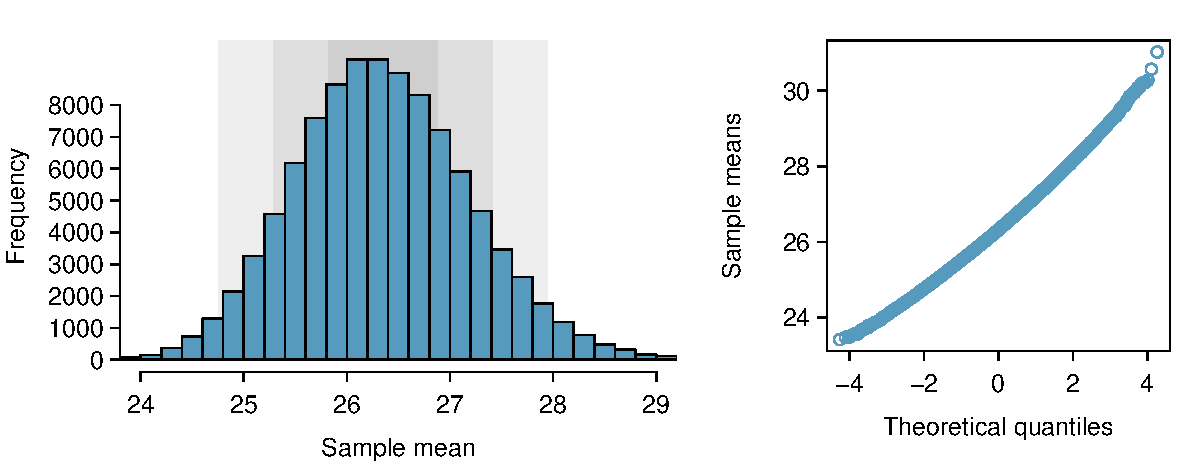
\includegraphics[width=\textwidth]{ch_inference_foundations_oi_biostat/figures/sampDistNormal/sampDistNormal}
   \caption{The left panel shows a histogram of the sample means for 100,000 different random samples of size $n=100$. The right panel shows a normal probability plot of those sample means.}
   \label{sampDistNormal}
\end{figure}

Does this distribution look familiar (think back to Chapter 2 of probability distributions)? Hopefully so! The distribution of sample means closely resembles the normal distribution (see Section~\ref{normalDist}). A normal probability plot of these sample means is shown in the right panel of Figure~\ref{sampDistNormal}. Because all of the points closely fall around a straight line, we can conclude the distribution of sample means is nearly normal. This result can be explained by the Central Limit Theorem\footnote{A more formal definition coming soon.}.

\begin{termBox}{\tBoxTitle{Central Limit Theorem, informal description}
If a sample consists of at least 30 independent observations and the data are not strongly skewed, then the distribution of the sample mean is well approximated by a~normal model.\index{Central Limit Theorem}}
\end{termBox}

\subsubsection{Why 30?}
\label{why30}

We introduce the Central Limit Theorem uses this cutoff at 30 in this text but this cutoff varies from book to book  As a quick exercise both in statistical exploration but also more practice in algorithmic thinking, think about how you would visually test if 30 independent observations is a sufficient number of observations to approximate the distribution to a normal model. Let's use the \data{BRFSS} data to sample from like before. 

Again remember we are testing if the normal model is a good approximation for the the sampling distribution with a sample size of 30. Creating a sampling distribution for sample sizes of $n=5,10,20,30$ and overlaying a normal approximation on the histogram is a great guide. \footnote{Use the same code for creating a sampling distribution but vary the sample size. Then use the code: 
\var{hist(sample.means, freq=FALSE ) \\
curve(dnorm(x,mean=mean(sample.means), sd=sqrt(var(sample.means))), add = TRUE)} where the function \var{curve()} adds the normal curve on top of the histogram.}

In Figure ~\ref{cltThirty} we see the sampling distributions of the sample mean for sample sizes of 5, 10, 20 and 30. The curve on top is a normal density curve with the normal distribution $\mathcal{N}(\mu, \sigma)$ where $\mu$ is the mean of the sample means and $\sigma$ is the standard deviation of the sample means.
FIX THISSSSSS
\begin{figure}[hht] 
   \centering
   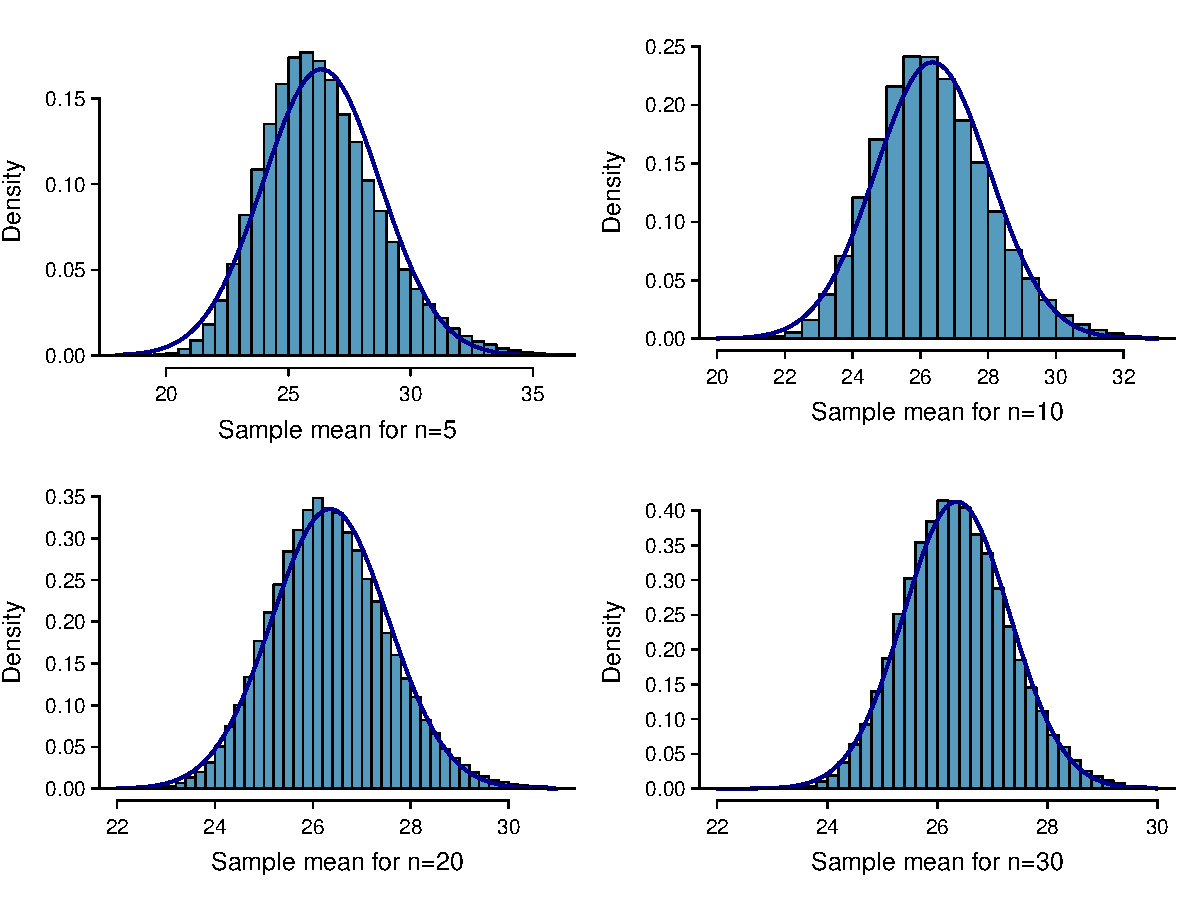
\includegraphics[width=\textwidth]{ch_inference_foundations_oi_biostat/figures/clt30/clt30}
     \label{cltThirty}
   \caption{The sampling distribution of sample means with different sample sizes $n=5, 10, 20, 30$. With a normal density curve on top, we see that for $n=30$, a normal model is a fitting approximation confirming the Central Limit Theorem rule of thumb.}
\end{figure}

We will apply this informal version of the Central Limit Theorem for now, and discuss its details further in Section~\ref{cltSection}.

The choice of using 2 standard errors in Equation~(\ref{95PercentConfidenceIntervalFormula}) was based on our general guideline that roughly 95\% of the time, observations are within two standard deviations of the mean. Under the normal model, with a sufficient number of samples ($n\geq 30$), we can make this more accurate by using 1.96 in place of  2.
\begin{eqnarray}
\text{point estimate}\ \pm\ 1.96\times SE
\label{95PercentCIWhenUsingNormalModel}
\end{eqnarray}
If a point estimate, such as $\bar{x}$, is associated with a normal model with standard error $SE$, then we use this more precise 1.96 to create a  95\% confidence interval. 

\subsection{Changing the confidence level}
\label{changingTheConfidenceLevelSection}

\index{confidence interval!confidence level|(}
6 Changing the confidence level
? Motivation: Sometimes your problem parameters don?t need you to be 95% confident. Sometimes (for
example with life threatening tests) you need to be more confident. Solution: you can change your
confidence level.



We have only discussed confidence intervals at the 95\% confidence level. Some situations, however, require conclusions to be more than 95\% confident. Consider a test for diagonosing a deathly disease in which doctors need to be more accurate. Perhaps we would like a confidence level of 99\%. There are also some scenarios where the problem parameters only require you to be 90\%

want to consider confidence intervals where the confidence level is somewhat higher than 95\%. Perhaps we would like a confidence level of 99\% or even lower like 90\%. Think back to the analogy about trying to catch a fish: if we want to be more sure that we will catch the fish, we should use a wider net. To create a 99\% confidence level, we must also widen our 95\% interval. On the other hand, if we want an interval with lower confidence, such as 90\%, we could make our original 95\% interval slightly slimmer.

The 95\% confidence interval structure provides guidance in how to make intervals with new confidence levels. Below is a general 95\% confidence interval for a point estimate where the point estimate follows a nearly normal distribution.
\begin{eqnarray}
\text{point estimate}\ \pm\ 1.96\times SE
\end{eqnarray}

There are three components to this interval: the point estimate, the ``1.96'', and the standard error.  The $1.96\times SE$ value affects the confidence interval width, and the point estimate affects where the confidence interval will be centered. Since we know from a normal distribution's Z-score that approximately 95\% of data that is normally distributed falls within 1.96 standard deviations of the mean, $1.96\times SE$ represents the width required to "capture that 95\%" of the sampling distribution as seen in Figure ~\ref{choosingZForCI}. 
 
\begin{exercise} \label{leadInForMakingA99PercentCIExercise}
If $X$ is a normally distributed random variable, how often will $X$ be within 2.58 standard deviations of the mean?\footnote{This is equivalent to asking how often the $Z$ score will be larger than -2.58 but less than 2.58. (For a picture, see Figure~\ref{choosingZForCI}.) To determine this probability, look up -2.58 and 2.58 in the normal probability table (0.0049 and 0.9951). Thus, there is a $0.9951-0.0049 \approx 0.99$ probability that the unobserved random variable $X$ will be within 2.58 standard deviations of $\mu$.}
\end{exercise}

\begin{figure}
\centering
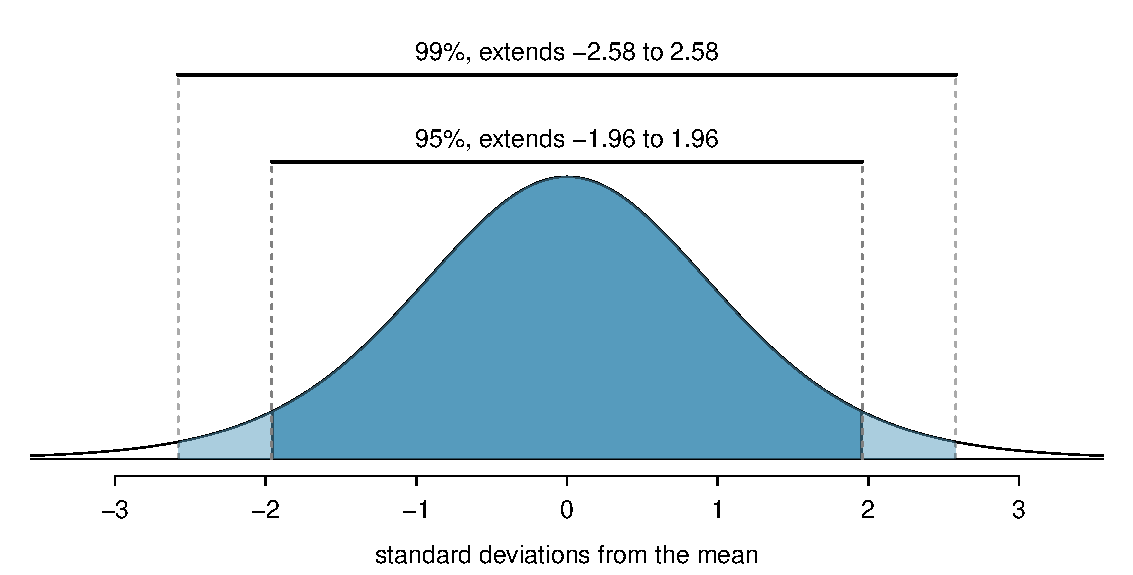
\includegraphics[width=\textwidth]{ch_inference_foundations_oi_biostat/figures/choosingZForCI/choosingZForCI}
\label{choosingZForCI}
\caption{The area between -$z^{\star}$ and $z^{\star}$ increases as $|z^{\star}|$ becomes larger. If the confidence level is 99\%, we choose $z^{\star}$ such that 99\% of the normal curve is between -$z^{\star}$ and $z^{\star}$, which corresponds to 0.5\% in the lower tail and 0.5\% in the upper tail: $z^{\star}=2.58$.}
\index{confidence interval!confidence level|)}
\end{figure}


To 99\% confident, change 1.96 in the 95\% confidence interval formula to be $2.58$ for a 99\% confidence interval. Exercise~\ref{leadInForMakingA99PercentCIExercise} highlights that 99\% of the time a normal random variable will be within 2.58 standard deviations of the mean. This approach -- using the Z scores in the normal model to compute confidence levels -- is appropriate when $\bar{x}$ is associated with a normal distribution with mean $\mu$ and standard deviation $SE_{\bar{x}}$. Thus, the formula for a 99\% confidence interval is
\begin{eqnarray}
\bar{x}\ \pm\ 2.58\times SE_{\bar{x}}
\label{99PercCIForMean}
\end{eqnarray}

The normal approximation is crucial to the precision of these confidence intervals. Section~\ref{cltSection} provides a more detailed discussion about when the normal model can safely be applied. When the normal model is not a good fit, we will use alternative distributions that better characterize the sampling distribution. Below however is a good checklist to determine whether or not the Central Limit Theorem can be informally applied to the distribution of sampling mean.

\begin{termBox}{\tBoxTitle{Conditions for $\bar{x}$ being nearly normal and $SE$ being accurate\label{terBoxOfCondForXBarBeingNearlyNormalAndSEBeingAccurate}}
Important conditions to help ensure the sampling distribution of $\bar{x}$ is nearly normal and the estimate of SE sufficiently accurate:
\begin{itemize}
\setlength{\itemsep}{0mm}
\item The sample observations are independent.
\item The sample size is large: $n\geq30$ is a good rule of thumb.
\item The population distribution is not strongly skewed. (We check this using the sample distribution as an estimate of the population distribution.)
\end{itemize}
Additionally, the larger the sample size, the more lenient we can be with the sample's skew.}
\end{termBox}

These three conditions help ensure that $\bar{x}$ is both distributed normally and representative of the target population. If the distribution of $\bar{x}$ is nearly normal, choosing a precise "1.96" or "2.58" becomes much easier for calculating confidence intervals. More importantly, however, the representativeness of the sample is imperative in our ability to infer about the target population. Randomness, independence and a large sample size safeguard against an extreme observation from skewing the conclusions from our sample. These conditions ensure the ability to accurately infer and generalize about the population of interest.

Verifying independence is often the most difficult of the conditions to check, and the way to check for independence varies from one situation to another. However, we can provide simple rules for the most common scenarios. 

\begin{tipBox}{\tipBoxTitle{How to verify sample observations are independent}
Observations in a simple random sample consisting of less than 10\% of the population are independent.}
\end{tipBox}

\begin{caution}
{Independence for random processes and experiments}
{If a sample is from a random process or experiment, it is important to verify the observations from the process or subjects in the experiment are nearly independent and maintain their independence throughout the process or experiment. Usually subjects are considered independent if they undergo random assignment in an experiment or are selected randomly for some process.}
\end{caution}

\begin{exercise} \label{find99CIForBRFSSWeightExercise}
Create a 99\% confidence interval for the average weight of men from the \data{brfss.sample} sample. The point estimate is $\bar{w} = 189.4$ and the standard error is $SE_{\bar{y}} = 0.178$. Refer to Figure ~\ref{brfssSampHist} for guidance on skewness.
\begin{figure}
\centering
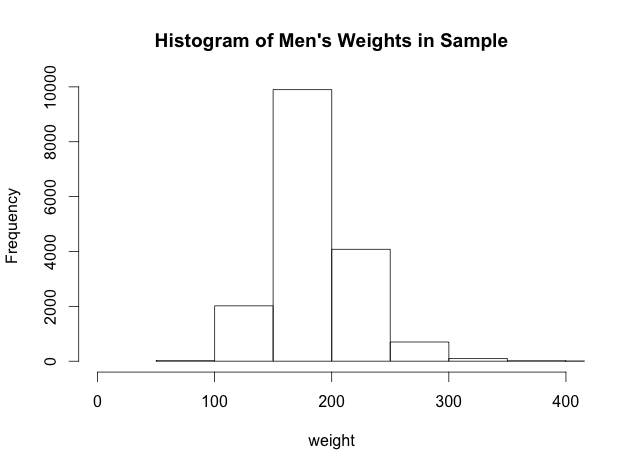
\includegraphics[width=0.75\textwidth]{ch_inference_foundations_oi_biostat/figures/choosingZForCI/brfssSampHist.png}
\caption{We draw a histogram of the men's weights in the \var{brfss.sample} and note that it is only slightly skewed. With 40,000 observations however, its skewness is more negligible because of its large sample size.}
\label{brfssSampHist}
\index{confidence interval!confidence level|)}
\end{figure}
\footnote{The observations are independent (simple random sample, $<10\%$ of the population), the sample size is at least 30 ($n=100$), and the distribution is only slightly skewed (Figure~\ref{brfssSampHist}); the normal approximation and estimate of SE should be reasonable.  Apply the 99\% confidence interval formula: $\bar{y}\ \pm\ 2.58 \times  SE_{\bar{y}} \rightarrow (188.94, 189.87)$. We are 99\% confident that the average weight of all males is between 188.94 and 189.87 pounds.}
\end{exercise}
%library(openintro); data(run10Samp); d <- run10Samp; mean(d$age); sd(d$age)/sqrt(100)

Now that we know how to calculate a 95\% and 99\% confidence interval given a nearly normally distributed $\bar{x}$, we can generalize this setup to any confidence level we choose. Remember while it has become tradition to use the 95\% confidence level, any confidence level is allowed and vary by statistician and by goal. 

\begin{termBox}{\tBoxTitle{Confidence interval for any confidence level (nearly normal model)}
If the point estimate follows the normal model with standard error $SE$, then a confidence interval for the population parameter is
\begin{eqnarray*}
\text{point estimate}\ \pm\ z^{\star} SE
\end{eqnarray*}
where $z^{\star}$ corresponds to the confidence level selected. The coefficient on the standard error, $z^{\star}$, is also known as the critical value. Remember that $z^{\star}$ is only used when the point estimate resembles a normal model \footnote{$z^{\star}$ is also used when the population standard deviation is known. However since we previously mentioned that this is rarely ever the case in practice, we have disregarded this situation completely}}
\end{termBox}
\begin{termBox}{\tBoxTitle{Margin of error}
\label{marginOfErrorTermBox}In a confidence interval, $z^{\star}\times SE$ is called the \term{margin of error}.}
\end{termBox}

Figure ~\ref{choosingZForCI} provides a picture of how to identify $z^{\star}$ based on a confidence level. We select $z^{\star}$ so that the area between -$z^{\star}$ and $z^{\star}$ in the normal model corresponds to the confidence level. We note from Figure~\ref{choosingZForCI} that the $z^{\star}$ value comes from a $\mathcal{N}(0,1)$. Therefore we can either use $R$ or a Z-table \footnote{also known as a Normal table} (\textbf{FOUND IN THE BACK OF THE BOOK HERE}) to find the critical value associated with some confidence level. In $R$, we use the \var{qnorm()} function. \var{qnorm()} takes in a probability $p$ and outputs the quantile value $z$ such that $P(Z\leq z)=p$. For a 95\% confidence interval, $p=0.025$ since we are looking for the \emph{middle} 95\%. Therefore in $R$\begin{verbatim}
> qnorm(0.025)
[1] -1.959964
\end{verbatim}
and we show that $z^{\star}=1.96$ is the critical value for 95\%. 
\begin{exercise} 
What is the critical value associated with (a) 90\%, (b) 75\% and (c) 50\%? \footnote{Remember we want the \emph{middle} and for any given confidence level $C$, we type into $R$, \var{qnorm($0.5\cdot (1-C)$)}. Therefore (a) \var{qnorm(0.05)= -1.644854} so $z^{\star}=1.65$ for a 90\% confidence level (b) 1.15 (c) 0.67}
\end{exercise}

\begin{exercise} \label{find90CIForBRFSSWeightExercise}
Use the data in Exercise~\ref{find99CIForBRFSSWeightExercise} to create a 90\% confidence interval for the average weight of men in the United States.\footnote{We first find $z^{\star}$ such that 90\% of the distribution falls between -$z^{\star}$ and $z^{\star}$ in the standard normal model, $N(\mu=0, \sigma=1)$. We can look up -$z^{\star}$ in the normal probability table by looking for a lower tail of 5\% (the other 5\% is in the upper tail), thus $z^{\star}=1.65$. The 90\% confidence interval can then be computed as $\bar{y}\ \pm\ 1.65\times SE_{\bar{y}} \to (189.11, 189.69)$. (We had already verified conditions for normality and the standard error in the previous exercise.) That is, we are 90\% confident the average weight of males is between 189.11 and 189.69 pounds. Also note that because we are at a 90\% confidence level, our confidence interval width is smaller than in Exercise ~\ref{find99CIForBRFSSWeightExercise}.}
\end{exercise}

\subsection{Interpreting confidence intervals}
\label{interpretingCIs}

\index{confidence interval!interpretation|(}

A careful eye might have observed the somewhat awkward language used to describe confidence intervals. Correct interpretation:
\begin{quote}
We are XX\% confident that the population parameter is between...
\end{quote}

Looking back to \textbf{Section 4.2.2}, this means that if we took a random sample from our population 100 times and calculated a confidence interval around our point estimate each time, 95 confidence intervals would contain the true population parameter. 

It is interesting to note, however, that researchers in practice would almost never be able to resample 100 times and generate 100 confidence intervals. The meaning of being "95\% confident" has traditionally been one grounded in theory and less in practice. "Confidence" relates more to the reliability of the process of creating such a range and less so in the probability that the value is within the range. 

\emph{Incorrect} language might try to describe the confidence interval as capturing the population parameter with a certain probability. This is one of the most common errors: while it might be useful to think of it as a probability, the confidence level only quantifies how plausible it is that the parameter is in the interval. 

Another especially important consideration of confidence intervals is that they \emph{only try to capture the population parameter}. Our intervals say nothing about the confidence of capturing individual observations, a proportion of the observations, a percent of all the data or just the sampled data. A confidence interval also says nothing about capturing point estimates since the confidence interval is always centered at the observed point estimate.  Confidence intervals only attempt to capture population parameters as statistical inference's goal is to infer about such population parameters.

Some incorrect interpretations of a 95\% confidence interval include: 
\begin{quote}
95\% of the observed data is between ...\\
95\% of the population distribution is contained in the confidence interval.\\
\end{quote}

Remember, a confidence interval is not a range of plausible values for the sample mean, though it may be understood as an estimate of plausible values for the population parameter.
A particular confidence interval of 95\% calculated from an experiment does not mean that there is a 95\% probability of a sample mean from a repeat of the experiment falling within this interval.[13]

While the differences in correct and incorrect interpretations are extremely nuanced, the goal of this book is to provide the tools and mechanisms of calculating and computing a confidence interval from data and less so about the wording which, in practice, has become almost meaningless and obsolete. 

\index{confidence interval!interpretation|)}
\index{confidence interval|)}

\subsection[Nearly normal population with known SD (special topic)]{Nearly normal population with known SD (special topic)}
\label{nearlyNormalPopWithKnownSD}

\index{Central Limit Theorem!normal data|(}

In rare circumstances we know important characteristics of a population. For instance, we might already know a population is nearly normal and we may also know its parameter values. Even so, we may still like to study characteristics of a random sample from the population. Consider the conditions required for modeling a sample mean using the normal distribution:
\begin{enumerate}
\setlength{\itemsep}{0mm}
\item[(1)] The observations are independent.
\item[(2)] The sample size $n$ is at least 30.
\item[(3)] The data distribution is not strongly skewed.
\end{enumerate}
These conditions are required so we can adequately estimate the standard deviation of the population from our sample and so we can ensure the distribution of sample means is nearly normal. However, if the population is known to be nearly normal, we know that the sample mean is always nearly normal (this is a special case of the Central Limit Theorem). If the standard deviation for the population is also known, then conditions (2) and (3) are not necessary for those data. 

We would like to heavily emphasize however that while, in practice, the population mean is more likely to be known, the population standard deviation is rarely know. While a known population standard deviation will rarely occur in practice, the Central Limit Theorem allows us to describe the distribution of the sampling distribution more specifically. 

\begin{example}{The heights of male seniors in high school closely follow a normal distribution $N(\mu=70.43, \sigma=2.73)$, where the units are inches.\footnote{These values were computed using the USDA Food Commodity Intake Database.} If we randomly sampled the heights of five male seniors, what distribution should the sample mean follow?}\label{simpleSampleOfFiveMaleSeniors}
The population is nearly normal, the population standard deviation is known, and the heights represent a random sample from a much larger population, satisfying the independence condition. Therefore the sample mean of the heights will follow a nearly normal distribution with mean $\mu=70.43$ inches and standard error $SE=\sigma/\sqrt{n} = 2.73/\sqrt{5}=1.22$ inches.
\end{example}

\begin{termBox}{\tBoxTitle{Alternative conditions for applying the normal distribution to model the sample mean}
If the population of cases is known to be nearly normal and the population standard deviation $\sigma$ is known, then the sample mean $\bar{x}$ will follow a nearly normal distribution $N(\mu, \sigma/\sqrt{n})$ if the sampled observations are also independent.}
\end{termBox}

Sometimes the mean changes over time but the standard deviation remains the same. In such cases, a sample mean of small but nearly normal observations paired with a known standard deviation can be used to produce a confidence interval for the current population mean using the normal distribution.

\begin{tipBox}{\tipBoxTitle{Relaxing the nearly normal condition}
As the sample size becomes larger, it is reasonable to \emph{slowly} relax the nearly normal assumption on the data when dealing with small samples. By the time the sample size reaches 30, the data must show strong skew for us to be concerned about the normality of the sampling distribution.}
\index{Central Limit Theorem!normal data|)}
\end{tipBox}

%__________________
\section{Hypothesis testing}
\label{hypothesisTesting}

\index{hypothesis testing|(}

Is the average US adult satisfied with his or her weight? We consider this question in the context of the \data{BRFSS} dataset comparing US adults' current weight and their desired weight (we will call this "weight difference"). While media pressures women to maintain a slim figure, the same media urges men to work out more and become stronger and more fit. These opposing viewpoints and many others all are components that influence satisfaction with weight and the desire to lose or gain weight. 

In addition to considering weight in this section, we consider a topic near and dear to most students: sleep. A recent study found that college students average about 7 hours of sleep per night.\footnote{\urlwofont{http://theloquitur.com/?p=1161}} However, researchers at a rural college are interested in showing that their students sleep longer than seven hours on average. We investigate this topic in Section~\ref{pValue}.

Many questions, given the correct data, can be answered through Hypothesis Testing. \term{Hypothesis testing} is a method in statistics that evaluates whether or not a population parameter has a hypothesized value with an associated probability of error. It is, most obviously, determining the probability that a given hypothesis is true or not.

Hypotheses are often simple questions that have a yes or no answer. Consider some hypotheses below: \begin{quote}
Is the mean body temperature really 98.6F? \\
Has consumption of soda changed across the US overtime? \\
Do MCAT classes improve MCAT scores? 
\end{quote}

The hypothesis testing process consists of generally 5 steps. Going through the \term{Hypothesis testing framework} allows for statisticians to answer these yes/no questions with a certain degree of confidence after observing a related sample. We begin by testing a hypothesis about a population mean from observing one sample. Remember, we can do hypothesis testing on any population parameter. It can be the population mean, population standard deviation or even the population IQR if desired. 

\subsection{Hypothesis testing framework}
\label{hypothesisFramework}

The average weight difference that adults want to experience that we observe from our sample of the \data{brfss.sample} data is 15.01 lbs. We want to determine if this sample provides enough evidence that adults are satisfied with their weight versus the alternative -- that they are not.\footnote{While we could answer this question by examining the entire population data (\data{BRFSS}), we only consider the sample data (\data{brfss.sample}), which is more realistic since statisticians rarely have access to population data.} We use desired weight difference as a proxy for weight satisfaction and simplify this question into two \termsub{hypotheses}: 
\begin{itemize}
\setlength{\itemsep}{0mm}
\item[$H_0$:] US adults are satisfied with their current weight. The average desired weight difference for US adults is 0 lbs. 
\item[$H_A$:] The average adult's desired weight difference is not 0 lbs i.e. Average adults are not satisfied with their current weights and would like to change. 
\end{itemize}

\subsubsection{Step 1: Formulating Hypotheses}

The first step within the hypothesis testing framework is setting up the hypotheses. As shown above, we generally have two hypotheses, a null and an alternative. 

We call $H_0$\marginpar[\raggedright\vspace{6mm}

$H_0$\\\footnotesize null hypothesis\vspace{3mm}\\\normalsize $H_A$\\\footnotesize alternative\\ hypothesis]{\raggedright\vspace{6mm}

$H_0$\\\footnotesize null hypothesis\vspace{3mm}\\\normalsize $H_A$\\\footnotesize alternative\\ hypothesis} the null hypothesis and $H_A$ the alternative hypothesis.

\begin{termBox}{\tBoxTitle{Null and alternative hypotheses}
{\small The \term{null hypothesis ($H_0$)} often represents either a skeptical perspective or a claim to be tested. The \term{alternative hypothesis ($H_A$)} represents an alternative claim under consideration and is often represented by a range of possible parameter values.}}
\end{termBox}

The null hypothesis often represents a skeptical position. The null hypothesis is generally denoted as "no difference" or what one would observe if there is no change.  The alternative hypothesis often represents a new perspective, such as the possibility that there has been a change. If the null hypothesis is true, any difference between the observed sample is due only to chance variation. 

\begin{tipBox}{\tipBoxTitle{Hypothesis testing framework}
The logic of hypothesis testing is that we will not reject the null hypothesis ($H_0$), unless the evidence in favor of the alternative hypothesis ($H_A$) is so strong that we must reject $H_0$ in favor of $H_A$.}
\end{tipBox}

The first step within the hypothesis testing framework is a very general tool, and we often use it without a second thought. If a person makes a somewhat unbelievable claim, we are initially skeptical. We believe our null hypothesis $H_0$. However, if there is sufficient evidence that we observe that supports the claim, we set aside our skepticism and reject the null hypothesis in favor of the alternative. 

\begin{exercise} \label{hypTestStudyExample}
A new study would like to be published in a scientific journal. The board that determines the validity of the study considers two possible claims about this study: either the study is valid or pseudoscience. If we set these claims up in a hypothesis framework, which would be the null hypothesis and which the alternative? \footnote{The board considers whether the study's evidence, results and reproducibility is so convincing (strong) that there the study must be valid. In this case the board rejects the null hypothesis (the study is pseudoscience) and concludes that the study is valid an should be published (alternative hypothesis).}
\end{exercise}

Those scientists who sit on the board of publication journals look at the study, previous literature and other evidence to see whether it convincingly supports that the science is valid. Even if these scientists leave unconvinced that the study is publishable, this does not mean that these board members believe the study is complete fabrication. This is also the case with hypothesis testing: \emph{even if we fail to reject the null hypothesis, we typically do not accept the null hypothesis as true}. Failing to find strong evidence for the alternative hypothesis is not equivalent to accepting the null hypothesis.

\begin{tipBox}{\tipBoxTitle{Double negatives can sometimes be used in statistics}
In many statistical explanations, we use double negatives. For instance, we might say that the null hypothesis is \emph{not implausible} or we \emph{failed to reject} the null hypothesis. Double negatives are used to communicate that while we are not rejecting a position, we are also not saying it is correct.}
\end{tipBox}

In the example with the \data{BRFSS} data, the null hypothesis represents no change in desired weight difference. The alternative hypothesis represents something new or more interesting: there was a difference, either a desire to gain or lose weight on average. These hypotheses can be described in mathematical notation using $\mu_{wd}$ as the average weight difference for US adults. 
\[H_0:\mu_{wd} = 0 \hspace{0.5in} H_A: \mu_{wd} \neq 0\]

where 0 represents a desired weight difference of 0 lbs or that these US adults on average do not care to change their weight. Using this mathematical notation, the hypotheses can now be evaluated using statistical tools. We call 0 the \term{null value} since it represents the value of the parameter if the null hypothesis is true. We will use the \data{brfss.sample} data set to evaluate the hypothesis test.

Note it is important to remember that we are not testing whether or not the average weight difference observed from the \data{brfss.sample} is 0 or not. We don't need to test that since we have observed all of \data{brfss.sample} and can simply calculate it. Rather we are testing the \emph{population parameter} or the true average value of all US adults' weight differences is 0 or not. 

\begin{tipBox}{\tipBoxTitle{Null and Alternative Hypothesis Setup}
The null hypothesis is generally written as $H_0: \mu=\mu_0$ where $\mu$ is the population mean and $\mu_0$ is the hypothesized value that we believe to be true.\\ The alternative hypothesis, on the other hand, can be many things.\\ If we have no prior belief to influence our alternative hypothesis and the researchers are interested in showing any difference --an increase or decrease-- then the safest one would be $\mu\neq \mu_0$ or a two-sided alternative. If we have a prior belief of how $\mu$ and $\mu_0$ compare or are interested in only showing an increase or decrease, but not both, we can do a one-sided alternative, $\mu\geq \mu_0$ or $\mu \leq \mu_0$. We will go into more detail on one-side versus two sided in Section ~\ref{pValue}.}
\end{tipBox}

\subsubsection{Step 2: Specifying a Significance Level $\alpha$}
Once we have completed Step 1 and have a null and alternative hypothesis, we need to specify a \term{significance level}. The significance level $\alpha$ is the acceptable error probability of the test.
In this case, the error probability is the probability of concluding the alternative hypothesis is true when it is not
true. This error is called a Type I error, and $\alpha$ is the probability of a Type I error. We will go into more detail on error types in Section \ref{DecisionErrors}. 

Typically, $\alpha$ is taken to be 0.05, 0.01, or some other small value. $\alpha$ plays the same role as the error probability in confidence intervals, and is a measure of uncertainty. If $\alpha=0.05$, we are testing at a 95\% confidence level for our hypothesis tests. We will see a clearer connection between hypothesis testing and confidence intervals in Section ~\ref{utilizingOurCI}. 

\subsubsection{Step 3: Calculating the Test Statistic}
The third step is calculating a test statistic from the data we observe. This statistic will be the value that the conclusions will be based on and measures the difference between the observed data and what is expected if the null hypothesis is true. This test statistic answers the question: "How many standard deviations from the hypothesized value is the observed sample value?" Thinking back to \textbf{THIS SECTION} ~\ref{some section} by standardizing a normal, the test statistic follows a similar construction. When testing hypotheses about a mean, the test statistic for the population mean from one sample will always be \[T=\frac{\bar{x}-\mu_0}{s/\sqrt{n}}\] where $\bar{x}$ is the sample mean, $s$ is the sample standard deviation and $n$ is the number of observations in the sample.
\emph{Note:} In general we see that test statistics follow $\frac{\mathrm{observed-hypothesized}}{\mathrm{standard error}}$ to see how many standard deviations the observed value is from the hypothesized value. 
This T-statistic follows a t-distribution \footnote{ from \textbf{Chapter 3}} and will have $n-1$ degrees of freedom. 

\begin{termBox}{\tBoxTitle{Test statistic}
A \emph{test statistic} is a special summary statistic that is particularly useful for evaluating a hypothesis test or identifying the p-value. The test-statistic is a particular data summary that summarizes how many standard deviations from the hypothesized null value is the observed sample value. In general the T-statistic follows a t-distribution with $n-1$ degrees of freedom. \footnote{When a point estimate is nearly normal, we use the Z score of the point estimate as the test statistic. In later chapters we encounter situations where other test statistics are helpful.}}
\index{hypothesis testing!using normal model|)}
\end{termBox}

\subsubsection{Step 4: Calculating the p-value}
Once we calculate a test statistic from the observed data, we know how many standard deviations our observation is from the hypothesized value if the null hypothesis were true. Now we need to tie this T-statistic value to a probability of such an observation happening. We do this through the \term{p-value}. Assuming the null hypothesis is true, the p-value is the probability of observing our sample or a more extreme sample. Formally the p-value is a conditional probability.

\begin{termBox}{\tBoxTitle{p-value}
The \term{p-value}\index{hypothesis testing!p-value|textbf} is the probability of observing data at least as favorable to the alternative hypothesis as our current data set, if the null hypothesis is true. We typically use a summary statistic of the data, in this chapter the sample mean, to help compute the p-value and evaluate the hypotheses.}
\end{termBox}

How do we get this probability? Section ~\ref{pValue} will go into more detail from using $R$, Z and t- tables. 

\subsubsection{Step 5: Making your conclusion}
The final step within the hypothesis testing framework is to make a conclusion from the p-value we calculated in Step 4. Using the definition of p-value, if we observe something extreme, the probability associated with our observation will be small. Thus if our observation is rare, the T-statistic and p-value provide evidence that the hypothesized value is unlikely. Therefore if our p-value is low, we should reject our null hypothesis, and the smaller the p-value, the stronger the evidence we have against the null hypothesis. 

How small is small? This is where Step 2 and our significance level comes in. If the p-value is small or smaller than the pre-specified $\alpha$ level (usually 0.01 or 0.05),  we reject the null hypothesis and say the result that we observe is statistically significant at the $\alpha$ level. 

If the p-value is $\alpha$ or greater, we simply do not have enough evidence to reject the null hypothesis. The subtle but important point is that not rejecting $H_0$ is not equivalent to accepting $H_0$ (refer back to Example \ref{hypTestStudyExample}). In practice, however, not rejecting $H_0$ is equivalent to accepting $H_0$ when making decisions and acting on conclusions. Most importantly, it is key that students state the conclusion in the context of the original problem, using the language and units of that problem. Most students forget this but is absolutely necessary in both theory and practice. 


\subsection{Calculating p-values}
\label{pValue}

\index{hypothesis testing!p-value|(}

Calculating p-values can be the most difficult part of the hypothesis testing framework. The p-value depends on many moving parts, including the sample mean, the sample size and the alternative hypothesis but always remember that the p-value is the probability of observing data as extreme or more if we assume the null hypothesis is true with the data at least as favorable to the alternative hypothesis. If the p-value is small, then our sample indicates that we just observed something rare, so rare that we should probably reject the null hypothesis as true. Figure~\ref{pValueOneSidedSleepStudyExplained} shows the distribution of the sample mean where the p-value is the shaded area for a one sided alternative $\mu > \mu_0$. 

\begin{figure}[ht]
   \centering
   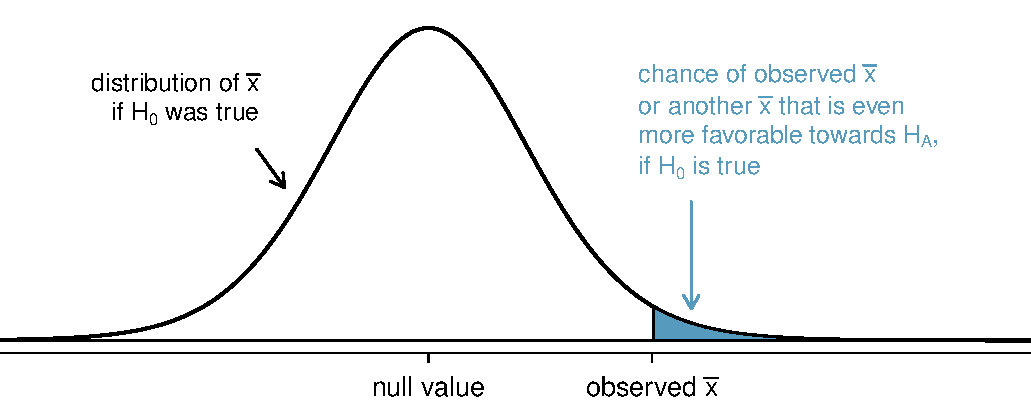
\includegraphics[width=0.9\textwidth]{ch_inference_foundations_oi_biostat/figures/pValueOneSidedSleepStudyExplained/pValueOneSidedSleepStudyExplained}
   \caption{To identify the p-value, the distribution of the sample mean is considered as if the null hypothesis was true. Then the p-value is defined and computed as the probability of observing the observed $\bar{x}$ or an $\bar{x}$ even more extreme and thus favorable to follow $H_A$ under this distribution.} 
   \label{pValueOneSidedSleepStudyExplained}
\end{figure}

If the alternative is one sided and has the form $\mu > \mu_0$, then the p-value would be represented by the upper tail (Figure~\ref{pValueOneSidedSleepStudyExplained}). If the alternative is one sided but has the form $\mu < \mu_0$, then the p-value would be the shaded area in the lower tail. In a two-sided test, \emph{we shade two tails} since evidence in either direction is favorable to $H_A$ (Figure ~\ref{2ndSchSleepHTExample}). 

\begin{figure}
   \centering
   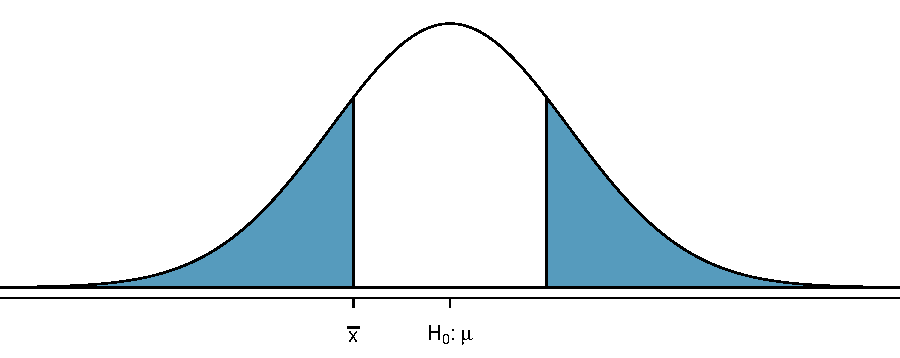
\includegraphics[width=0.9\textwidth]{ch_inference_foundations_oi_biostat/figures/2ndSchSleepHTExample/2ndSchSleepHTExample}
   \caption{$H_A$ is two-sided, so \emph{both} tails must be counted for the p-value.}
   \label{2ndSchSleepHTExample}
\end{figure}

Now that we know what the p-value represents, how do we actually get this shaded area to be a number? Here is where the T-statistic comes into play. Before we get to the nitty gritty, let's look back to the \data{BRFSS} data. 

Recall that the researchers for the \data{BRFSS} data are interested if US adults are satisfied with their current weight. They believe that the desired weight difference is a good proxy to measure satisfaction and have the following null and alternative hypotheses where $\mu_{wd}$ denotes the average desired weight difference in the US: 

 \begin{itemize}
\setlength{\itemsep}{0mm}
\item[$H_0$:] $\mu_{wd}=0$
\item[$H_A$:] $\mu_{wd} \neq 0$ 
\end{itemize}

Instead of 40,000 within our sample, let's say that we observed a sample of 100 people and calculated a sample mean of weight differences of 0.5 pounds and standard deviation of 5 pounds. Given this information we can first calculate a T-statistic\footnote{calculating the T-statistic using actual data is an exercise in the book}. \[t=\frac{0.5-0}{25/\sqrt{100}}= 0.2\] The T-statistic can be thought of as a Z-score (standard score) that indicates how many standard deviations the observed sample mean is from the null value. This standardization becomes a great way to unify all the moving parts in order to calculate the p-value. 

With the T-statistic and the alternative hypothesis, we calculate the p-value from either a t-distribution or a normal distribution. The sample size determines which distribution to model our point estimate from, either a t-distribution or a normal distribution. If $n \geq 30$ \textbf{from this part}, the sample mean can be thought of coming from a normal distribution. If $n < 30$, model the sampling distribution from a t-distribution. 

With $\alpha=0.05$, students can either use a table to calculate the p-value or use $R$. First assuming a t-distribution, use the t-table given \textbf{on some page} to find the row with the correct degrees of freedom (in a one sample test, $df=n-1$). Students then should look across that row to find the T-statistic value that they calculated. Note that the table won't have every single value listed but once they find the approximate T-statistic, look at the top of the column to get p-value using either a one sided or two sided (one tail or two tail) alternative. The normal table (Z-table) is very similar but be wary of that the Z-table only lists the areas left of the Z-score. This simply means that these probabilities coincide with a one-sided alternative. However because the normal distribution is symmetric, finding the p-value for a two sided alternative is just those values from the table times two! 

If available, $R$ is also a handy tool. Use the \var{pt()} or the \var{pnorm()} function to calculate the area left of the T-statistic. Students then can take the value and subtract from one or multiply by two depending on the alternative hypothesis. If students have the ability to use $R$, the $n\geq 30$ threshold can be loosened since modeling after the t-distribution becomes easier and more accurate compared to the tables. However we note again that once $n\geq 30$, both distributions become almost equal. 

We use a normal table for calculating the p-value for our sample from the \data{BRFSS} data because $n=100$  in our sample. A score of 0.2 corresponds to a shaded area of 0.579 to the left. Therefore in the tail we have 
\begin{align*}
p &=Pr(T\leq -0.2) + Pr(T\geq 0.2)\\
&= Pr(|T| \geq 0.2)\\
&= 2Pr(T\geq 0.2)\\
&= 2 \cdot (1-0.579)\\
&= 0.842
\end{align*}
Using $R$, we use both \var{pnorm()} and \var{pt()} to check. \begin{verbatim}
> 2*(1-pnorm(0.2))
[1] 0.8414806
> 2*(1-pt(0.2, 99))
[1] 0.8418908
\end{verbatim}

We see that both output p-values that are extremely similar and agree with the p-value from the normal table as well. Now that we calculated the p-value we can conclude that this p-value $> \alpha=0.05$ so we cannot reject $H_0$. To put it into context: from observing a sample mean of 0.5 for weight differences, we observed a p-value of 0.84 and cannot conclude that weight difference is nonzero. From our sample it appears that US adults are satisfied with their weight. 

\begin{exercise}
If the null hypothesis is true, how often should the p-value be less than 0.05?\footnote{About 5\% of the time. If the null hypothesis is true, then the data only has a 5\% chance of being in the 5\% of data most favorable to $H_A$.}
\index{data!school sleep|)}
\end{exercise}

\begin{tipBox}{\tipBoxTitle{Concluding on Critical Values}
Conclusions are made from the p-value but if $\alpha=0.05$ or some other common value, we can take a quick shortcut using the critical value. We learned the critical value as the coefficient on the standard error to calculate the confidence interval. However the critical value is also the point on the test distribution that can be compared to the T-statistic in hypothesis testing. Since we know that the critical value is associated with some confidence level, this critical value is also associated with $\alpha$. If the absolute value of the T-statistic is greater than the critical value (more extreme), the p-value is less than $\alpha$ and you can reject the null hypothesis.}
\end{tipBox}

\begin{caution}{Critical value $\neq$ test statistic}
{Many times students get confused between the critical value and the test statistic. The critical value is associated with some $\alpha$ and does not change. For a specific $\alpha$ there is only one critical value. The T-statistic can change depending on the sample that you observed. Students are comparing their T-statistic to the critical value using the critical value as a benchmark.} 
\end{caution}

\begin{exercise} \label{skepticalPerspOfRuralSchoolSleepExercise}
A poll by the National Sleep Foundation found that college students average about 7 hours of sleep per night. Researchers at a rural school are interested in showing that students at their school sleep longer than seven hours on average, and they would like to demonstrate this using a sample of students. What would be an appropriate skeptical position for this research?\footnote{A skeptic would have no reason to believe that sleep patterns at this school are different than the sleep patterns at another school.}
\end{exercise}

\index{data!school sleep|(}

We can set up the null hypothesis for this test as a skeptical perspective: the students at this school average 7 hours of sleep per night. The alternative hypothesis takes a new form reflecting the interests of the research: the students average more than 7 hours of sleep. We can write these hypotheses as
\[H_0: \mu = 7 \hspace{0.5in} H_A: \mu \geq 7\]
Using $\mu \geq 7$ as the alternative is an example of a \term{one-sided} hypothesis test mentioned previously. In this investigation, there is no apparent interest in learning whether the mean is less than 7~hours.\footnote{This is entirely based on the interests of the researchers. Had they been only interested in the opposite case -- showing that their students were actually averaging fewer than seven hours of sleep but not interested in showing more than 7 hours -- then our setup would have set the alternative as $\mu \leq 7$.} Earlier we encountered a \term{two-sided} hypothesis where we looked for any clear difference, greater than or less than the null value.

Always use a two-sided test unless it was made clear prior to data collection that the test should be one-sided. Switching a two-sided test to a one-sided test after observing the data is dangerous because it can inflate the chance of an incorrect conclusion.

\begin{tipBox}{\tipBoxTitle{One-sided and two-sided tests}
If the researchers are only interested in showing an increase or a decrease, but not both, use a one-sided test. If the researchers would be interested in any difference from the null value -- an increase or decrease -- then the test should be two-sided.\vspace{0.5mm}}
\end{tipBox}

\begin{tipBox}{\tipBoxTitle{Always write the null hypothesis as an equality}
We will find it most useful if we always list the null hypothesis as an equality (e.g. $\mu = 7$) while the alternative always uses an inequality (e.g. $\mu\neq7$, $\mu \geq7$, or $\mu \leq7$).}
\end{tipBox}

The researchers at the rural school conducted a simple random sample of $n=110$ students on campus. They found that these students averaged 7.42 hours of sleep and the standard deviation of the amount of sleep for the students was 1.75 hours. A histogram of the sample is shown in Figure~\ref{histOfSleepForCollegeThatWasCheckingForMoreThan7Hours}.

\begin{figure}
\centering
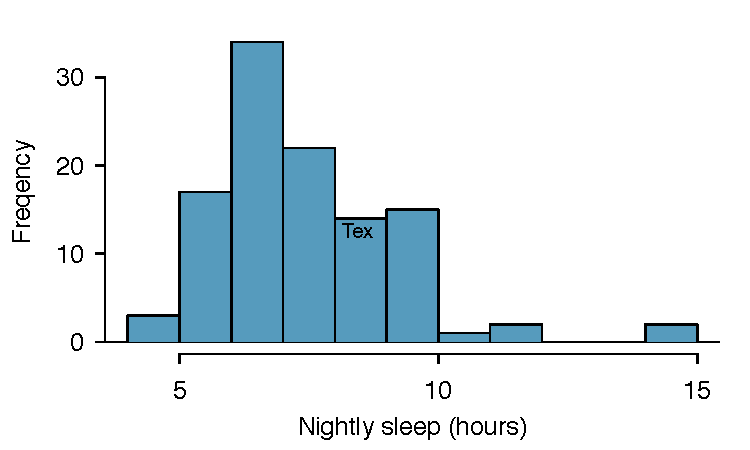
\includegraphics[height=55mm]{ch_inference_foundations_oi_biostat/figures/histOfSleepForCollegeThatWasCheckingForMoreThan7Hours/histOfSleepForCollegeThatWasCheckingForMoreThan7Hours}
\caption{Distribution of a night of sleep for 110 college students. These data are moderately skewed.\index{skew!example: moderate}}
\label{histOfSleepForCollegeThatWasCheckingForMoreThan7Hours}
\end{figure}

Before we can use a normal model for the sample mean or compute the standard error of the sample mean, we must verify conditions. (1)~Because this is a simple random sample from less than 10\% of the student body, the observations are independent. (2)~The sample size in the sleep study is sufficiently large since it is greater than 30. (3)~The data show moderate skew in Figure~\ref{histOfSleepForCollegeThatWasCheckingForMoreThan7Hours} and the presence of a couple of outliers. This skew and the outliers (which are not too extreme) are acceptable for a sample size of $n=110$. With these conditions verified, the normal model can be safely applied to $\bar{x}$ and the estimated standard error will be very accurate.

\begin{exercise} \label{findSEOfFirstSleepStudyCheckingGreaterThan7Hours}
What is the standard deviation associated with $\bar{x}$? That is, estimate the standard error of $\bar{x}$.\footnote{The standard error can be estimated from the sample standard deviation and the sample size: $SE_{\bar{x}} = \frac{s_x}{\sqrt{n}} = \frac{1.75}{\sqrt{110}} = 0.17$.}
\end{exercise}

The hypothesis test will be evaluated using a significance level of $\alpha = 0.05$. We want to consider the data under the scenario that the null hypothesis is true. In this case, the sample mean is from a distribution that is nearly normal and has mean 7 and standard deviation of about 0.17. Such a distribution is shown in Figure~\ref{pValueOneSidedSleepStudy}. 

\begin{figure}[hht]
   \centering
   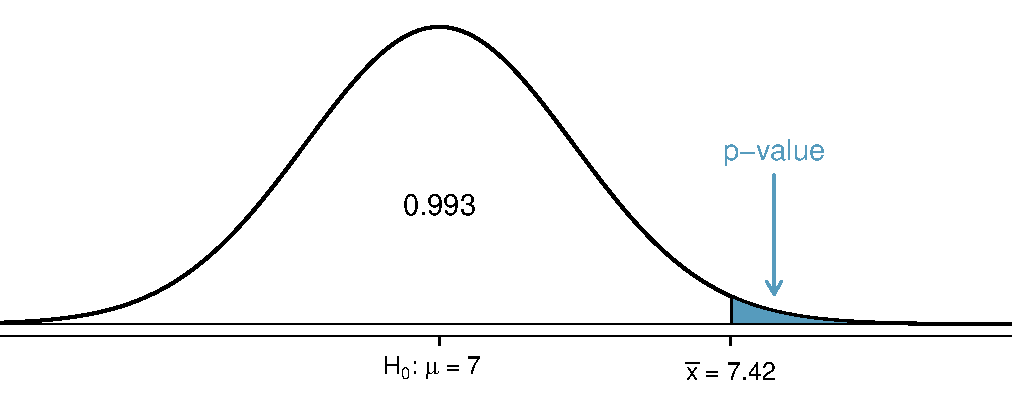
\includegraphics[width=0.73\textwidth]{ch_inference_foundations_oi_biostat/figures/pValueOneSidedSleepStudy/pValueOneSidedSleepStudybrfss}
   \caption{If the null hypothesis is true, then the sample mean $\bar{x}$ came from this nearly normal distribution. The right tail describes the probability of observing such a large sample mean if the null hypothesis is true.}
   \label{pValueOneSidedSleepStudy}
\end{figure}

Remember the shaded tail in Figure~\ref{pValueOneSidedSleepStudy} is the p-value and so we shade all means larger than our sample mean, $\bar{x} = 7.42$, because they are more favorable to the alternative hypothesis than the observed mean. We compute the p-value by first computing the T-statistic for the sample mean, $\bar{x} = 7.42$:
\[ T = \frac{\bar{x} - \text{null value}}{SE_{\bar{x}}} = \frac{7.42 - 7}{0.17} = 2.47\]

Using the normal probability table, the lower unshaded area is found to be 0.993. Thus the shaded area is $1-0.993 = 0.007$. Using $R$ we have
 \begin{verbatim} 
 > 1-pnorm(2.47)
[1] 0.006755653 
\end{verbatim}
{\em If the null hypothesis is true, the probability of observing such a large sample mean for a sample of 110 students is only 0.007.}\index{p-value!interpretation example} That is, if the null hypothesis is true, we would not often see such a large mean.

We evaluate the hypotheses by comparing the p-value to the significance level. Because the p-value is less than the significance level (p-value $=0.007 < 0.05=\alpha$), we reject the null hypothesis.\footnote{Using critical values instead, we know that for $\alpha=0.05$ and a one sided alternative, the critical value is 1.65. Since our T-statistic is greater than 1.65, we know to reject $H_0$ without calculating the actual p-value} What we observed is so unusual with respect to the null hypothesis that it casts serious doubt on $H_0$ and provides strong evidence favoring $H_A$.

\begin{termBox}{\tBoxTitle{p-value as a tool in hypothesis testing}
The p-value quantifies how strongly the data favor $H_A$ over $H_0$. A small p-value (usually $<0.05$) corresponds to sufficient evidence to reject $H_0$ in favor of $H_A$.}
\index{hypothesis testing!p-value|)}
\end{termBox}

\begin{tipBox}{\tipBoxTitle{It is useful to first draw a picture to find the p-value}
It is useful to draw a picture of the distribution of $\bar{x}$ as though $H_0$ was true (i.e. $\mu$ equals the null value), and shade the region (or regions) of sample means that are at least as favorable to the alternative hypothesis. These shaded regions represent the p-value.}
\end{tipBox}

\begin{exercise}
Suppose we had used a significance level of 0.01 in the sleep study. Would the evidence have been strong enough to reject the null hypothesis? (The p-value was 0.007.) What if the significance level was $\alpha = 0.001$? \footnote{We reject the null hypothesis whenever $p$-$value < \alpha$. Thus, we would still reject the null hypothesis if $\alpha = 0.01$ but not if the significance level had been $\alpha = 0.001$.}
\end{exercise}

\subsection{Testing hypotheses using confidence intervals}
\label{utilizingOurCI}

While confidence intervals may appear separate from hypothesis testing, these two concepts arrive as the same conclusions. Consider a sample of 100 people from the \data{BRFSS} data to test if the average age of adults is 36.8 years \footnote{as calculated by the US Census in 2009}. The hypothesis setup would be $H_0: \mu_{\mathrm{age}}=36.8$ and $H_A: \mu_{\mathrm{age}} \neq 36.8$. We learned in Section~\ref{variabilityInEstimates} that there is fluctuation from one sample to another, and it is very unlikely that the sample mean will be exactly equal to our parameter; we should not expect $\bar{x}_{\mathrm{ages}}$ to exactly equal $\mu_{\mathrm{ages}}$ and the difference could be due to \emph{sampling variation}, i.e. the variability associated with the point estimate when we take a random sample.

In Section~\ref{confidenceIntervals}, confidence intervals were introduced as a way to find a range of plausible values for the population mean. From \data{BRFSS}, the sample has a mean of 46.48 and a standard deviation of 16.83. Therefore the 95\% confidence interval is \[46.48 \pm 1.96 \cdot \frac{16.83}{\sqrt{100}} = (43.1796, 49.7804)\] Because 36.8 years does not fall in the range of plausible values, we can say the null hypothesis is implausible. That is, we failed to reject the null hypothesis, $H_0$. 

\begin{exercise} \label{htForHousingExpenseForCommunityCollege650}
An investigator is studying the results of standardized IQ tests in adolescents who suffered from severe asthma during childhood. She claims that those who had childhood asthma perform worse. For the standardized test she will use, the population mean score is 100. What are the null and alternative hypotheses to test whether this claim is accurate? \footnote{$H_0$: The average score is 100, $\mu = 100$. \hspace{3.4mm} $H_A$: The average score is lower, $\mu \leq 100$.}
\end{exercise}

\begin{example}{In her sample of 100 children, she found a sample mean $\bar{x} = 96.7$ and standard deviation $s = 10$. Construct a 95\% confidence interval for the population mean and evaluate the hypotheses of Exercise~\ref{htForHousingExpenseForCommunityCollege650}.}
$$ SE = \frac{s}{\sqrt{n}} = \frac{10}{\sqrt{100}} = 1 $$
The normal model may be applied to the sample mean because the conditions are met: The data are a simple random sample and we assume that there are more than 1,000 adolescents who have suffered from asthma. The observations are independent and the sample size is also sufficiently large (n=100). We don't know about existing outliers but the sample size mitigates potential effects of outliers. This ensures a 95\% confidence interval may be accurately constructed:
$$\bar{x}\ \pm\ z^{\star} SE \quad\to\quad 96.7\ \pm\ 1.96 \times  1 \quad \to \quad (94.74, 98.66) $$
Because the null value 100 is not in the confidence interval, a true mean of 100 is implausible and we reject the null hypothesis. The data provide statistically significant evidence that adolescents who suffered from severe asthma during childhood do perform worse on standardized IQ tests. 
\end{example}

\subsection{Decision errors}\label{DecisionErrors}

\index{hypothesis testing!decision errors|(}

Hypothesis tests are not flawless. Just think of the court system: innocent people are sometimes wrongly convicted and the guilty sometimes walk free. Similarly, we can make a wrong decision in statistical hypothesis tests. However, the difference is that we have the tools necessary to quantify how often we make such errors.

There are two competing hypotheses: the null and the alternative. In a hypothesis test, we make a statement about which one might be true, but we might choose incorrectly. There are four possible scenarios in a hypothesis test, which are summarized in Table~\ref{fourHTScenarios}.

\begin{table}[ht]
\centering
\begin{tabular}{l l c c}
& & \multicolumn{2}{c}{\textbf{Test conclusion}} \\
  \cline{3-4}
\vspace{-3.7mm} \\
& & do not reject $H_0$ &  reject $H_0$ in favor of $H_A$ \\
  \cline{2-4}
\vspace{-3.7mm} \\
& $H_0$ true & okay &  Type~1 Error \\
\raisebox{1.5ex}{\textbf{Truth}} & $H_A$ true & Type 2 Error & okay \\
  \cline{2-4}
\end{tabular}
\caption{Four different scenarios for hypothesis tests.}
\label{fourHTScenarios}
\end{table}

A \term{Type~1 Error} is rejecting the null hypothesis when $H_0$ is actually true. A \term{Type~2 Error} is failing to reject the null hypothesis when the alternative is actually true.

\begin{exercise} \label{whatAreTheErrorTypesInUSCourts}
In a US court, the defendant is either innocent ($H_0$) or  guilty ($H_A$). What does a Type~1 Error represent in this context? What does a Type 2 Error represent? Table~\ref{fourHTScenarios} may be useful.\footnote{If the court makes a Type~1 Error, this means the defendant is innocent ($H_0$ true) but wrongly convicted. A Type 2 Error means the court failed to reject $H_0$ (i.e. failed to convict the person) when she was in fact guilty ($H_A$ true).}
\end{exercise}

\begin{exercise} \label{howToReduceType1ErrorsInUSCourts}
How could we reduce the Type~1 Error rate in US courts? What influence would this have on the Type 2 Error rate?\footnote{To lower the Type~1 Error rate, we might raise our standard for conviction from ``beyond a reasonable doubt'' to ``beyond a conceivable doubt'' so fewer people would be wrongly convicted. However, this would also make it more difficult to convict the people who are actually guilty, so we would make more Type~2 Errors.}
\end{exercise}

\begin{exercise} \label{howToReduceType2ErrorsInUSCourts}
How could we reduce the Type~2 Error rate in US courts? What influence would this have on the Type~1 Error rate?\footnote{To lower the Type~2 Error rate, we want to convict more guilty people. We could lower the standards for conviction from ``beyond a reasonable doubt'' to ``beyond a little doubt''. Lowering the bar for guilt will also result in more wrongful convictions, raising the Type~1 Error rate.}
\end{exercise}

\begin{exercise} \label{errorsinHIVTesting}
Consider a person getting tested for HIV. What does a Type~1 and Type~2 Error represent in this context? \footnote{Type~1 Error is if this person does not have HIV but was tested positive for HIV. Type~2 Error would be failing to detect HIV when the patient actually has HIV. }
\end{exercise}

\index{hypothesis testing!decision errors|)}

Exercises~\ref{whatAreTheErrorTypesInUSCourts}-\ref{howToReduceType2ErrorsInUSCourts} provide an important lesson: if we reduce how often we make one type of error, we generally make more of the other type.

Hypothesis testing is built around rejecting or failing to reject the null hypothesis. That is, we do not reject $H_0$ unless we have strong evidence. But what precisely does \emph{strong evidence} mean? As a general rule of thumb, for those cases where the null hypothesis is actually true, we do not want to incorrectly reject $H_0$ more than 5\% of the time. This corresponds to a \term{significance level}\index{hypothesis testing!significance level} of 0.05 which is the same significance level from hypothesis testing and confidence intervals. We often write the significance level using $\alpha$\marginpar[\raggedright\vspace{-4mm}

$\alpha$\\\footnotesize significance\\level of a\\hypothesis test]{\raggedright\vspace{-4mm}

$\alpha$\\\footnotesize significance\\level of a\\hypothesis test} where $\alpha = 0.05$. We discuss the appropriateness of different significance levels in Section~\ref{significanceLevel}.

If we use a 95\% confidence interval to test a hypothesis where the null hypothesis is true, we will make an error whenever the point estimate is at least 1.96 standard errors away from the population parameter. This happens about 5\% of the time (2.5\% in each tail). Similarly, using a 99\% confidence interval to evaluate a hypothesis is equivalent to a significance level of $\alpha = 0.01$.

\subsection{Two-sided versus One-sided hypothesis testing: Dos and Don'ts}
\label{twoSidedTestsWithPValues}

\index{data!school sleep|(}

Determining an alternative hypothesis can get tricky, and the choice between a one-sided and two sided test can be controversial. In this book, the examples and exercises will be obvious enough to decide a correct alternative hypothesis. In practice with real world data, however, can be less straightforward. If the sidedness is uncertain, many scientists opt to use a two-sided alternative because it is more \emph{conservative}. What does conservative in this context mean? Let's first consider the differences.

It is never okay to change two-sided tests to one-sided tests after observing the data. In this example we explore the consequences of ignoring this advice. Using $\alpha=0.05$, we show that freely switching from two-sided tests to one-sided tests will cause us to make twice as many Type~1 Errors as intended. \footnote{hence to be conservative and safe, we opt to minimize the Type~1 Errors and use the two sided alternative}\label{swappingHypAfterDataDoublesType1ErrorRate}


\begin{exercise} \label{2ndSchSleepHypSetupExercise}
Earlier we talked about a research group investigating whether the students at their school slept longer than 7 hours each night. Let's consider a second group of researchers who want to evaluate whether the students at their college differ from the norm of 7 hours. Write the null and alternative hypotheses for this investigation.\footnote{Because the researchers are interested in any difference, they should use a two-sided setup: $H_0: \mu = 7$, $H_A: \mu \neq 7$.}
\end{exercise}

\begin{example}{The second college randomly samples 72 students and finds a mean of $\bar{x} = 6.83$ hours and a standard deviation of $s=1.8$ hours. Does this provide strong evidence against $H_0$ in Exercise~\ref{2ndSchSleepHypSetupExercise}? Use a significance level of $\alpha=0.05$.}
First, we must verify assumptions. (1) A simple random sample of less than 10\% of the student body means the observations are independent. (2) The sample size is 72, which is greater than 30. (3) Based on the earlier distribution and what we already know about college student sleep habits, the distribution is probably not strongly~skewed.

Next we can compute the standard error ($SE_{\bar{x}} = \frac{s}{\sqrt{n}} = 0.21$) of the estimate and create a picture to represent the p-value, shown in Figure~\ref{2ndSchSleepHTExample}. Both tails are shaded. An estimate of 7.17 ($6.83 + 1.65 cdot 0.21$) or more provides at least as strong of evidence against the null hypothesis and in favor of the alternative as the observed estimate, $\bar{x} = 6.83$.

We can calculate the tail areas by first finding the lower tail corresponding to $\bar{x}$:
\begin{eqnarray*}
T = \frac{6.83 - 7.00}{0.21} = -0.81 \quad\stackrel{table}{\rightarrow}\quad \text{left tail}=0.2090
\end{eqnarray*}
Because the normal model is symmetric, the right tail will have the same area as the left tail. The p-value is found as the sum of the two shaded tails:
\begin{eqnarray*}
\text{p-value} = \text{left tail} + \text{right tail} = 2\times(\text{left tail}) = 0.4180
\end{eqnarray*}
This p-value is relatively large (larger than $\alpha=0.05$), so we should not reject $H_0$. That is, if $H_0$ is true, it would not be very unusual to see a sample mean this far from 7 hours simply due to sampling variation. Thus, we do not have sufficient evidence to conclude that the mean is different than 7 hours.

\index{data!school sleep|)}

\begin{figure}
   \centering
   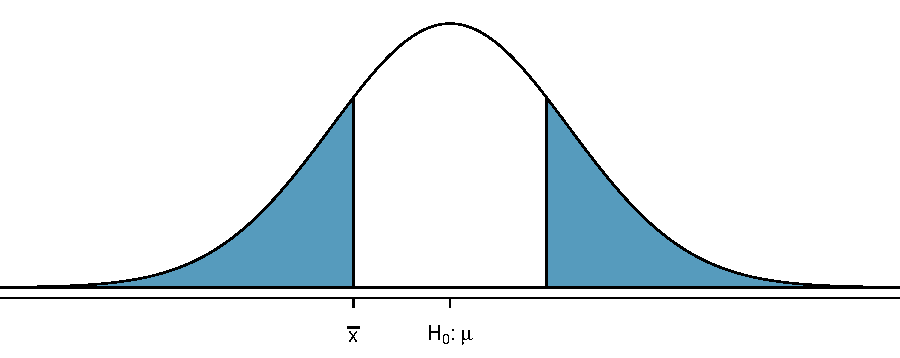
\includegraphics[width=0.9\textwidth]{ch_inference_foundations_oi_biostat/figures/2ndSchSleepHTExample/2ndSchSleepHTExample}
   \caption{$H_A$ is two-sided, so \emph{both} tails must be counted for the p-value.}
   \label{2ndSchSleepHTExample}
\end{figure}

\end{example}

\begin{example}{Let's consider two cases: (1) The sample mean was larger than the null value and (2) the sample mean as smaller than the null value. 

Suppose the sample mean was larger than the null value, $\mu_0$ (e.g. $\mu_0$ would represent~7 if $H_0$:~$\mu = 7$). Then if we can flip to a one-sided test instead of a two-sided test, we would use $H_A$: $\mu > \mu_0$. Now if we obtain any observation with a T-statistic greater than 1.65, we would reject $H_0$. If the null hypothesis is true, we incorrectly reject the null hypothesis about 5\% of the time when the sample mean is above the null value, as shown in Figure~\ref{type1ErrorDoublingExampleFigure}.

Suppose the sample mean was smaller than the null value. Then if we change to a one-sided test, we would use $H_A$: $\mu < \mu_0$. If $\bar{x}$ had a T-statistic smaller than -1.65, we would reject $H_0$. If the null hypothesis is true, then we would observe such a case about 5\% of the time.}

By examining these two scenarios, we can determine that we will make a Type~1 Error $5\%+5\%=10\%$ of the time if we are allowed to swap to the ``best'' one-sided test for the data. This is twice the error rate we prescribed with our significance level: $\alpha=0.05$! 

\begin{figure}
   \centering
   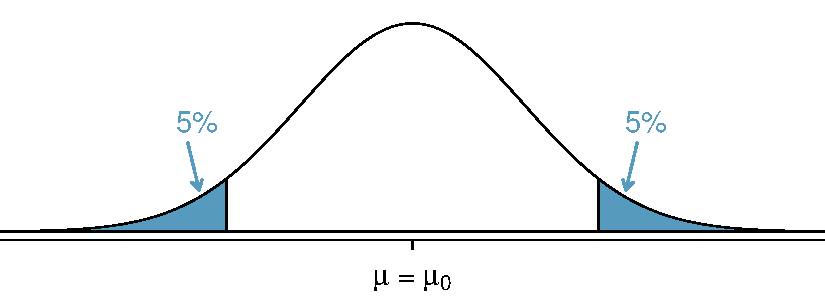
\includegraphics[width=0.7\textwidth]{ch_inference_foundations_oi_biostat/figures/type1ErrorDoublingExampleFigure/type1ErrorDoublingExampleFigure}
   \caption{The shaded regions represent areas where we would reject $H_0$ under the bad practices considered in Example~\ref{swappingHypAfterDataDoublesType1ErrorRate} when $\alpha = 0.05$.}
   \label{type1ErrorDoublingExampleFigure}
\end{figure}

\end{example}

\begin{caution}{One-sided hypotheses are allowed only \emph{before} seeing data}
{After observing data, it is tempting to turn a two-sided test into a one-sided test. Avoid this temptation. Remember, the direction of a one-sided test must be made a priori, not after peeking at the data since the results could be statistically significant with a one-sided test, but not significant with a two-sided test. Hypotheses must be set up \emph{before} observing the data. If~they are not, the test must be two-sided.}
\end{caution}

\subsection{Choosing a significance level}
\label{significanceLevel}

\index{hypothesis testing!significance level|(}
\index{significance level|(}

Choosing a significance level for a test is important in many contexts, and the traditional level is $\alpha=0.05$. However, it is often helpful to adjust the significance level based on the application. We may select a level that is smaller or larger than 0.05 depending on the consequences of any conclusions reached from the test.

If making a Type~1 Error is dangerous or especially costly, we should choose a small significance level (e.g. smaller than 0.05). Under this scenario we want to be very cautious about rejecting the null hypothesis, so we demand very strong evidence favoring $H_A$ before we would reject $H_0$. Many would use $\alpha=0.01$ in this situation. 

If a Type 2 Error is relatively more dangerous or much more costly than a Type~1 Error, then we should choose a higher significance level (e.g. 0.10). Here we want to be cautious about failing to reject $H_0$ when the null is actually false.  We will discuss this particular case in greater detail in Section~\ref{sampleSizeAndPower}.

\begin{tipBox}{\tipBoxTitle[]{Significance levels should reflect consequences of errors}
The significance level selected for a test should reflect the consequences associated with Type~1 and Type 2 Errors.}
\end{tipBox}

\begin{example}{A medical machine manufacturer is considering a higher quality but more expensive supplier for parts in making an MRI. They sample a number of parts from their current supplier and also parts from the new supplier. They decide that if the high quality parts will last more than 12\% longer, it makes financial sense to switch to this more expensive supplier. Is there good reason to modify the significance level in such a hypothesis test?}
The null hypothesis is that the more expensive parts last no more than 12\% longer while the alternative is that they do last more than 12\% longer. This decision is just one of the many regular factors that have a marginal impact on the MRI and the company financial health. A significance level of 0.05 seems reasonable since neither a Type~1 or Type 2 error should be dangerous or (relatively) much more expensive since the machine's accuracy won't be affected.
\end{example}

\begin{example}{Now consider that the same MRI manufacturer is considering a slightly more expensive supplier for parts related to safety not longevity. If the durability of the machine's components is shown to be better than the current supplier, they will switch manufacturers. Is there good reason to modify the significance level in such an evaluation?}
The null hypothesis would be that the suppliers' parts are equally reliable and equally accurate in detection. Because safety is involved, the MRI machine company should be eager to switch to the slightly more expensive manufacturer (reject $H_0$) even if the evidence of increased safety and effectiveness is only moderately strong. A slightly larger significance level, such as $\alpha=0.10$, might be appropriate.
\end{example}

\begin{exercise}
A part inside of a machine is very expensive to replace. However, the machine usually functions properly even if this part is broken and still detects the most common injuries at the same level with a fixed part. The part is replaced only if we are extremely certain it is broken based on a series of measurements. Identify appropriate hypotheses for this test (in plain language) and suggest an appropriate significance level.\footnote{Here the null hypothesis is that the part is not broken, and the alternative is that it is broken. If we don't have sufficient evidence to reject $H_0$, we would not replace the part. It sounds like failing to fix the part if it is broken ($H_0$ false, $H_A$ true) is not very problematic, and replacing the part is expensive. Thus, we should require very strong evidence against $H_0$ before we replace the part. Choose a small significance level, such as $\alpha=0.01$.}
\end{exercise}

\index{significance level|)}
\index{hypothesis testing!significance level|)}
\index{hypothesis testing|)}

%__________________
\section{Examining the Central Limit Theorem Closer (Special Topic)}
\label{cltSection}

\index{Central Limit Theorem|(}

Looking back to ~\ref{why30}, we discovered that the normal model for the sample mean tends to be very good when the sample consists of at least 30 independent observations and the population data are not strongly skewed. The Central Limit Theorem provides the theory that allows us to make this assumption.

\begin{termBox}{\tBoxTitle{Central Limit Theorem, informal definition}
The distribution of $\bar{x}$ is approximately normal. The approximation can be poor if the sample size is small, but it improves with larger sample sizes.}
\end{termBox}

The Central Limit Theorem states that when the sample size is small, the normal approximation may not be very good. However, as the sample size becomes large, the normal approximation improves. We will investigate three theoretical cases to see roughly when the approximation is reasonable.

We consider three data sets: one from a \emph{uniform} distribution, one from an \emph{exponential} distribution, and the other from a \emph{log-normal} distribution. Recall the properties of these distributions from Chapter ~\ref{modeling}. These distributions are shown in the top panels of Figure~\ref{cltSimulations}. The uniform distribution is symmetric, the exponential distribution may be considered as having moderate skew since its right tail is relatively short (few outliers), and the log-normal distribution is strongly skewed and will tend to produce more apparent outliers.\index{skew!example: moderate}\index{skew!example: strong}

\begin{figure}
   \centering
   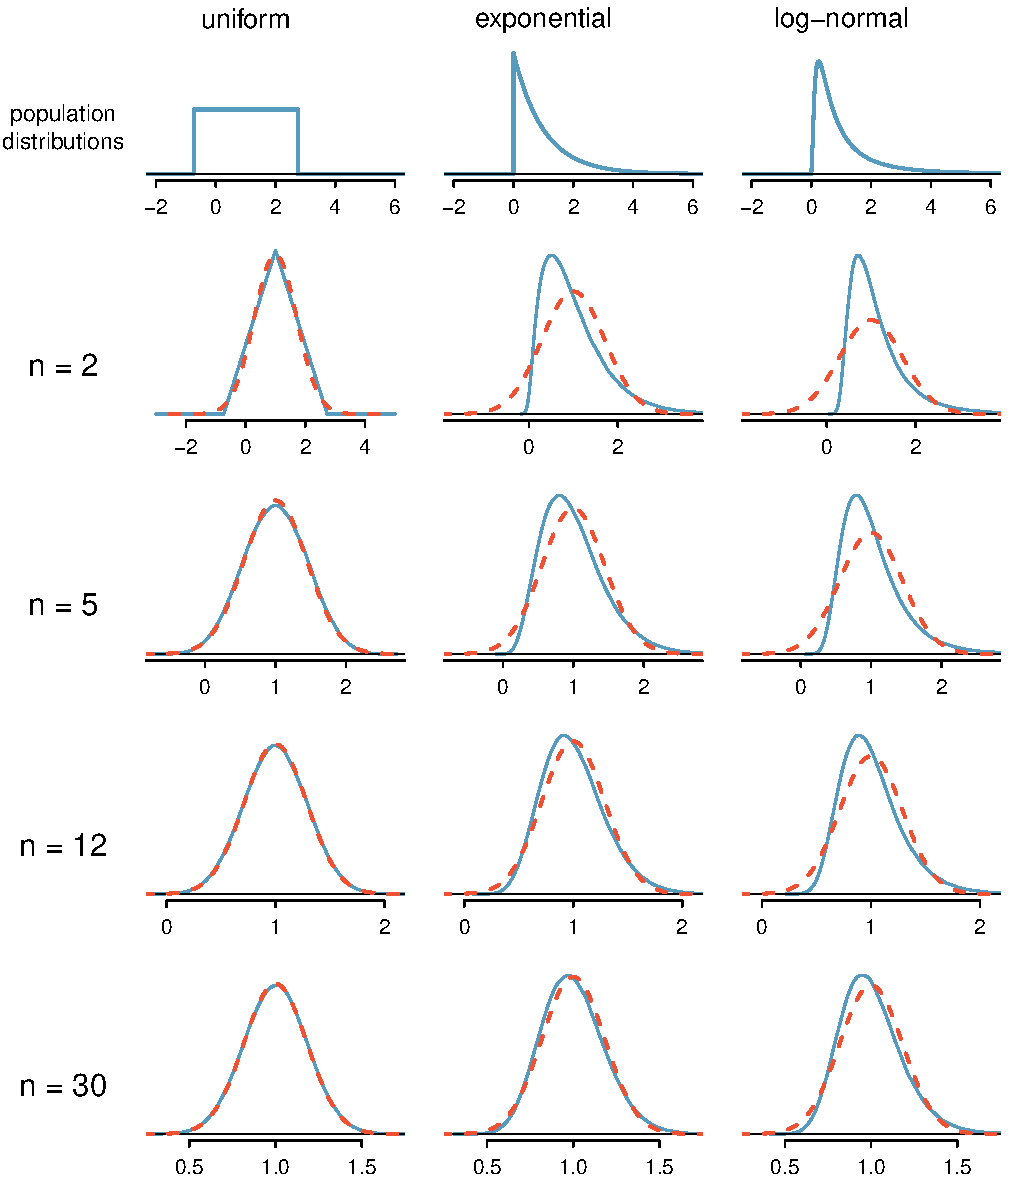
\includegraphics[width=\textwidth]{ch_inference_foundations_oi_biostat/figures/cltSimulations/cltSimulations}
   \caption{Sampling distributions for the mean at different sample sizes and for three different distributions. The dashed red lines show normal distributions.}
   \label{cltSimulations}
\end{figure}

The left panel in the $n=2$ row represents the sampling distribution of $\bar{x}$ if it is the sample mean of two observations from the uniform distribution shown. The dashed line represents the closest approximation of the normal distribution. Similarly, the center and right panels of the $n=2$ row represent the respective distributions of $\bar{x}$ for data from exponential and log-normal distributions.

\begin{exercise}
Examine the distributions in each row of Figure~\ref{cltSimulations}. What do you notice about the normal approximation for each sampling distribution as the sample size becomes larger?\footnote{The normal approximation becomes better as larger samples are used.}
\end{exercise}

\begin{example}{Would the normal approximation be good in all applications where the sample size is at least 30?}
Not necessarily. For example, the normal approximation for the log-normal example is questionable for a sample size of 30. Generally, the more skewed a population distribution or the more common the frequency of outliers, the larger the sample required to guarantee the distribution of the sample mean is nearly normal.
\end{example}

\begin{tipBox}{\tipBoxTitle{With larger $n$, the sampling distribution of $\bar{x}$ becomes more normal}
As the sample size increases, the normal model for $\bar{x}$ becomes more reasonable. We can also relax our condition on skew when the sample size is very large.}
\end{tipBox}

We discussed in Section~\ref{seOfTheMean} that the sample standard deviation, $s$, could be used as a substitute of the population standard deviation, $\sigma$, when computing the standard error. This estimate tends to be reasonable when $n\geq30$. We will encounter alternative distributions for smaller sample sizes in Chapters~\ref{inferenceForNumericalData} and~\ref{inferenceForCategoricalData}.



%%%%%%%%%%%%%%%%%THINK OF A NEW EXAMPLE. THIS IS A USEFUL TOPIC 
\begin{example}{Figure~\ref{pokerProfitsCanApplyNormalToSampMean} shows a histogram of 50 observations. These represent the number of patient visits in a hospital for 50 consecutive days relative to their average rate of 5000 patient visits. Can the normal approximation be applied to the sample mean, 90.69?}
We should consider each of the required conditions.
\begin{itemize}
\setlength{\itemsep}{0mm}
\item[(1)] These are referred to as \term{time series data}, because the data arrived in a particular sequence. Time series data generally deals with, you guessed it, time! If there are a lot of patients in the hospital one day, it may influence how many patients there are the day after. During the flu season, patient visits might be at an all time high since many people are sick but also the time per visit is also extremely low. To make the assumption of independence we should perform careful checks on such data. While the supporting analysis is not shown, no evidence was found to indicate the observations are not independent on a whole.
\item[(2)] The sample size is 50, satisfying the sample size condition.
\item[(3)] There are two outliers, one very extreme, which suggests the data are very strongly skewed or very distant outliers may be common for this type of data. Outliers can play an important role and affect the distribution of the sample mean and the estimate of the standard error.
\end{itemize}
Since we should be skeptical of the independence of observations and the very extreme upper outlier poses a challenge, we should not use the normal model for the sample mean of these 50 observations. If we can obtain a much larger sample, perhaps several hundred observations over a longer period of time, then the concerns about skew and outliers would no longer apply.
\end{example}

\begin{figure}[ht]
   \centering
   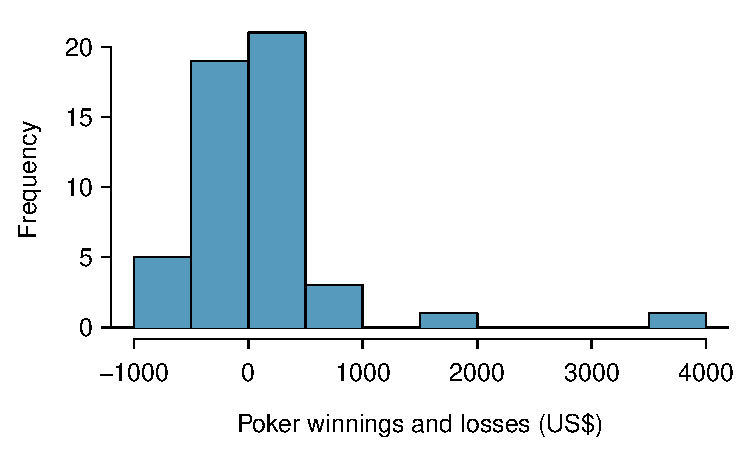
\includegraphics[height=58mm]{ch_inference_foundations_oi_biostat/figures/pokerProfitsCanApplyNormalToSampMean/pokerProfitsCanApplyNormalToSampMean}
   \caption{Sample distribution of total patient visits net of 5,000 visits. These data include some very clear outliers. These are problematic when considering the normality of the sample mean. For example, outliers are often an indicator of very strong skew\index{skew!example: very strong}.}
   \label{pokerProfitsCanApplyNormalToSampMean}
\end{figure}

\begin{caution}
{Examine data structure when considering independence}
{Some data sets are collected in such a way that they have a natural underlying structure between observations, e.g. when observations occur consecutively. Be especially cautious about independence assumptions regarding such data sets.}
\end{caution}

\begin{caution}
{Watch out for strong skew and outliers}
{Strong skew is often identified by the presence of clear outliers. If a data set has prominent outliers, or such observations are somewhat common for the type of data under study, then it is useful to collect a sample with many more than 30 observations if the normal model will be used for $\bar{x}$. There are no simple guidelines for what sample size is big enough for all situations, so proceed with caution when working in the presence of strong skew or more extreme outliers.}
\index{skew!strongly skewed guideline}
\index{Central Limit Theorem|)}
\end{caution}


%__________________
\section{Inference for other estimators}
\label{aFrameworkForInference}

The sample mean is not the only point estimate for which the sampling distribution is nearly normal. For example, the sampling distribution of sample proportions closely resembles the normal distribution when the sample size is sufficiently large. In this section, we introduce a number of examples where the normal approximation is reasonable for the point estimate. Chapters~\ref{inferenceForNumericalData} and~\ref{inferenceForCategoricalData} will revisit each of the point estimates you see in this section along with some other new statistics.

We make another important assumption about each point estimate encountered in this section: the estimate is unbiased. A point estimate is \term{unbiased} if the sampling distribution of the estimate is centered at the parameter it estimates. A biased point estimate on the other hand can always be too high or estimates always too low. That is, an unbiased estimate does not naturally over or underestimate the parameter. Rather, it tends to provide a ``good'' estimate. The sample mean is an example of an unbiased point estimate, as are each of the examples we introduce in this section.

Finally, we will discuss the general case where a point estimate may follow some distribution other than the normal distribution. We also provide guidance about how to handle scenarios where the statistical techniques you are familiar with are insufficient for the problem at hand.

\subsection{Confidence intervals for nearly normal point estimates}

\index{confidence interval!using normal model|(}

In Section~\ref{confidenceIntervals}, we used the point estimate $\bar{x}$ with a standard error $SE_{\bar{x}}$ to create a 95\% confidence interval for the population mean:
\begin{align}
\bar{x}\ \pm\ 1.96 \times SE_{\bar{x}}
\label{95PercCIForMeanInGeneralizingSection}
\end{align}
We constructed this interval by noting that the sample mean is within 1.96 standard errors of the actual mean about 95\% of the time. This same logic generalizes to any unbiased point estimate that is nearly normal. We may also generalize the confidence level by using a place-holder $z^{\star}$.

\begin{termBox}{\tBoxTitle{General confidence interval for the normal sampling distribution case}\label{generalConfidenceIntervalTermBox}%
For any unbiased point estimate, the confidence interval for a nearly normal point estimate is
\begin{eqnarray}
\text{point estimate}\ \pm\ z^{\star}SE
\label{95PercGeneralCIInGeneralizingSection}
\end{eqnarray}
We see that it is of the same form as the generalized confidence interval for the sample mean where $z^{\star}$ is selected to correspond to the confidence level, and $SE$ represents the standard error. Remember from previously that the value $z^{\star}SE$ is called the \emph{margin of error}\index{margin of error}.}
\end{termBox}

Generally the standard error for a point estimate is estimated from the data and computed using a formula. For example, the standard error for the sample mean is
\begin{eqnarray*}
SE_{\bar{x}} = \frac{s}{\sqrt{n}}
\end{eqnarray*}
In this section, we provide the computed standard error for each example and exercise without detailing where the values came from. In future chapters, you will learn to fill in these and other details for each situation.

\begin{example}{Using the \data{brfss.sample} data, we computed a point estimate for the average difference in weights between me and women: $\bar{x}_\mathrm{{men}}-\bar{x}_\mathrm{{women}}= 36.61162$ pounds. This point estimate is associated with a nearly normal distribution with SE = 0.35 pounds. What is a reasonable 95\% confidence interval for the difference in gender weights?}
\label{confIntervalForDifferenceOfRunTimeBetweenGenders}
The normal approximation is said to be valid, so we apply Equation~\eqref{95PercGeneralCIInGeneralizingSection}:
\begin{eqnarray*}
\text{point estimate}\ \pm\ z^{\star} SE
	\quad\rightarrow\quad 36.61\ \pm\ 1.96\times 0.35
	\quad\rightarrow\quad (35.91, 37.31)
\end{eqnarray*}
Thus, we are 95\% confident that the men were, on average, between 35.91 to 37.31 pounds heavier than women. That is, the actual average difference is plausibly between 35.91 and 37.31 pounds with 95\% confidence.
\end{example}
%library(openintro); library(xtable); data(run10); data(run10Samp); (x <- by(run10Samp$time, run10Samp$gender, mean)); diff(x); s <- by(run10Samp$time, run10Samp$gender, sd); n <- by(run10Samp$time, run10Samp$gender, length); sqrt(sum(s^2/n))


\begin{example}{Does Example~\ref{confIntervalForDifferenceOfRunTimeBetweenGenders} guarantee that if a husband and wife both weighted themselves, the husband would weigh between 35.91 and 37.31 pounds more than the wife?}
Our confidence interval says absolutely nothing about individual observations. It {only} makes a statement about a plausible range of values for the \emph{average} difference between all men and women in the US. 
\end{example}

\begin{exercise}
The proportion of men in the \data{brfss.sample} sample is $\hat{p}=0.42$. This sample meets certain conditions that ensure $\hat{p}$ will be nearly normal, and the standard error of the estimate is $SE_{\hat{p}}=0.05$. Create a 90\% confidence interval for the proportion of participants in the BRFSS study and thus in the US who are men.\footnote{We use $z^{\star}=1.65$, and apply the general confidence interval formula:
\begin{eqnarray*}
\hat{p}\ \pm\ z^{\star}SE_{\hat{p}}
	\quad\to\quad 0.42\ \pm\ 1.65\times 0.05
	\quad\to\quad (0.3375, 0.5025)
\end{eqnarray*}
Thus, we are 90\% confident that between 34\% and 50\% are men.}
\index{confidence interval!using normal model|)}
\end{exercise}


\subsection{Hypothesis testing for nearly normal point estimates}
\index{hypothesis testing!using normal model|(}

Just as the confidence interval method works with many other point estimates and we see the obvious connection between confidence intervals and hypothesis testing, it is unsurprising that we can generalize our hypothesis testing methods to new point estimates that are unbiased. Here we only consider the p-value approach, introduced in Section~\ref{pValue}. Remember the Hypothesis testing framework from ~\ref{hypothesisFramework}. 

\begin{termBox}{\tBoxTitle[]{Hypothesis testing framework using the normal model}
\begin{enumerate}
\setlength{\itemsep}{0mm}
\item First write the hypotheses in plain language, then set them up in mathematical notation using the appropriate point estimate and parameter of interest. 
\item State a significance level $\alpha$. We generally use $\alpha=0.05$. 
\item Compute the test-statistic using the point estimate and standard error estimate. 
\item Calculate the p-value by drawing a picture of the sampling distribution under $H_0$. Know which area you are shading to represent the correct p-value. 
\item Use the p-value to evaluate your hypotheses. Write a conclusion within the context of the problem. 
\end{enumerate}
} For point estimates other than the sampling mean which we know to be unbiased and nearly normal for $n>30$, students need to verify conditions to ensure that the point estimate is nearly normal and unbiased so that the standard error estimate is also reasonable. This step can be done before computing the test-statistic.  
\end{termBox}

\begin{exercise} \label{fdaHypSetupForSulph}
A drug called sulphinpyrazone was under consideration for use in reducing the death rate in heart attack patients. To determine whether the drug was effective, a set of 1,475 patients were recruited into an experiment and randomly split into two groups: a control group that received a placebo and a treatment group that received the new drug. What would be an appropriate null hypothesis? And the alternative?\footnote{The skeptic's perspective is that the drug does not work at reducing deaths in heart attack patients ($H_0$), while the alternative is that the drug does work ($H_A$).}
\end{exercise}

We can formalize the hypotheses from Exercise~\ref{fdaHypSetupForSulph} by letting $p_{control}$ and $p_{treatment}$ represent the proportion of patients who died in the control and treatment groups, respectively. Then the hypotheses can be written as
\begin{eqnarray*}
&&H_0: p_{control} = p_{treatment} \quad\text{(the drug doesn't work)} \quad \\
&&H_A: p_{control} > p_{treatment} \quad\text{(the drug works)}
\end{eqnarray*}
or equivalently,
\begin{eqnarray*}
&&H_0: p_{control} - p_{treatment} = 0 \quad\text{(the drug doesn't work)} \quad \\
&&H_A: p_{control} - p_{treatment} > 0 \quad\text{(the drug works)}
\end{eqnarray*}
Strong evidence against the null hypothesis and in favor of the alternative would correspond to an observed difference in death rates,
\begin{eqnarray*}
\text{point estimate} = \hat{p}_{control} - \hat{p}_{treatment}
\end{eqnarray*}
being larger than we would expect from chance alone. This difference in sample proportions represents a point estimate that is useful in evaluating the hypotheses. 

\begin{example}{We want to evaluate the hypothesis setup from Exericse~\ref{fdaHypSetupForSulph} using data from the actual study.\footnote{Anturane Reinfarction Trial Research Group. 1980. Sulfinpyrazone in the prevention of sudden death after myocardial infarction. New England Journal of Medicine 302(5):250-256.} In the control group, 60 of 742 patients died. In the treatment group, 41 of 733 patients died. The sample difference in death rates can be summarized as
\begin{eqnarray*}
\text{point estimate} = \hat{p}_{control} - \hat{p}_{treatment} = \frac{60}{742} - \frac{41}{733} = 0.025
\end{eqnarray*}
This point estimate is nearly normal and is an unbiased estimate of the actual difference in death rates. The standard error of this sample difference is $SE = 0.013$. Evaluate the hypothesis test at a 5\% significance level: $\alpha=0.05$.}
We would like to identify the p-value to evaluate the hypotheses. If the null hypothesis is true, then the point estimate would have come from a nearly normal distribution, like the one shown in Figure~\ref{sulphStudyFindPValueUsingNormalApprox}. The distribution is centered at zero since $p_{control}-p_{treatment}=0$ under the null hypothesis. Because a large positive difference provides evidence against the null hypothesis and in favor of the alternative, the upper tail has been shaded to represent the p-value. We need not shade the lower tail since this is a one-sided test: an observation in the lower tail does not support the alternative hypothesis.

\begin{figure}[bt]
   \centering
   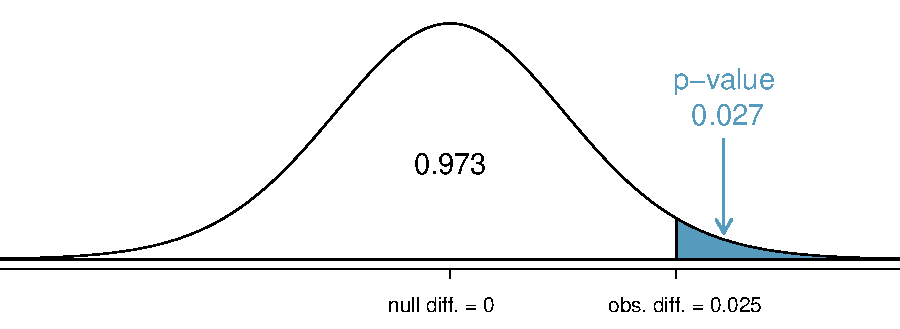
\includegraphics[height=37mm]{ch_inference_foundations_oi_biostat/figures/sulphStudyFindPValueUsingNormalApprox/sulphStudyFindPValueUsingNormalApprox}
   \caption{The distribution of the sample difference if the null hypothesis is true.}
   \label{sulphStudyFindPValueUsingNormalApprox}
\end{figure}

The p-value can be computed by using the Z score of the point estimate and the normal probability table.
\begin{eqnarray}
Z = \frac{\text{point estimate} - \text{null value}}{SE_{\text{point estimate}}}
	= \frac{0.025 - 0}{0.013} = 1.92
\label{zScoreOfPointEstimateForSulphinpyrazoneThisIsFirstTestStatReference}
\end{eqnarray}
Examining $Z$ in the normal probability table, we find that the lower unshaded tail is about 0.973. Thus, the upper shaded tail representing the p-value is
\begin{eqnarray*}
\text{p-value} = 1-0.973 = 0.027
\end{eqnarray*}
Because the p-value is less than the significance level ($\alpha=0.05$), we say the null hypothesis is implausible. That is, we reject the null hypothesis in favor of the alternative and conclude that the drug is effective at reducing deaths in heart attack patients.
\end{example}

\subsection{Non-normal point estimates}

We may apply the ideas of confidence intervals and hypothesis testing to cases where the point estimate or test statistic is not necessarily normal. There are many reasons why such a situation may arise:
\begin{itemize}
\setlength{\itemsep}{0mm}
\item the sample size is too small for the normal approximation to be valid;
\item the standard error estimate may be poor; or
\item the point estimate tends towards some distribution that is not the normal distribution.
\end{itemize}
For each case where the normal approximation is not valid, our first task is always to understand and characterize the sampling distribution of the point estimate or test statistic. Next, we can apply the general frameworks for confidence intervals and hypothesis testing to these alternative distributions.


\subsection{When to retreat}
\label{whenToRetreat}

Statistical tools rely on conditions. When the conditions are not met, these tools are unreliable and drawing conclusions from them is treacherous. The conditions for these tools typically come in two forms.
\begin{itemize}
\setlength{\itemsep}{0mm}
\item \textbf{The individual observations must be independent.} A random sample from less than 10\% of the population ensures the observations are independent. In experiments, we generally require that subjects are randomized into groups. If independence fails, then advanced techniques must be used, and in some such cases, inference may not be possible.
\item \textbf{Other conditions focus on sample size and skew.} For example, if the sample size is too small, the skew too strong, or extreme outliers are present, then the normal model for the sample mean will fail.
\end{itemize}
Verification of conditions for statistical tools is always necessary. Whenever conditions are not satisfied for a statistical technique, there are three options. The first is to learn new methods that are appropriate for the data. The second route is to consult a statistician.\footnote{If you work at a university, then there may be campus consulting services to assist you. Alternatively, there are many private consulting firms that are also available for hire.} The third route is to ignore the failure of conditions. This last option effectively invalidates any analysis and may discredit novel and interesting findings.

Finally, we caution that there may be no inference tools helpful when considering data that include unknown biases, such as convenience samples. For this reason, there are books, courses, and researchers devoted to the techniques of sampling and experimental design. See Sections~\ref{overviewOfDataCollectionPrinciples}-\ref{experimentsSection} for basic principles of data collection.



%__________________
\section{Sample size and power (special topic)}
\label{sampleSizeAndPower}

The Type 2 Error rate and the magnitude of the error for a point estimate are controlled by the sample size \footnote{Remember the margin of error comes from the confidence interval (point estimate $\pm$ margin of error where the margin of error = $q^{\star} \cdot SE$ for a certain confidence level)}. Real differences from the null value, even large ones, may be difficult to detect with small samples. If we take a very large sample, we might find a statistically significant difference but the magnitude might be so small that it is of no practical value. In this section we describe techniques for selecting an appropriate sample size based on these considerations.

\subsection{Finding a sample size for a certain margin of error}
\label{findingASampleSizeForACertainME}

\index{margin of error|(}

Many companies are concerned about rising healthcare costs. A company may estimate certain health characteristics of its employees, such as blood pressure, to project its future cost obligations. However, it might be too expensive to measure the blood pressure of every employee at a large company, and the company may choose to take a sample instead.

\begin{example}{Blood pressure oscillates with the beating of the heart, and the systolic pressure is defined as the peak pressure when a person is at rest. The average systolic blood pressure for people in the U.S. is about 130 mmHg with a standard deviation of about 25 mmHg. How large of a sample is necessary to estimate the average systolic blood pressure with a margin of error of 4 mmHg using a 95\% confidence level?}
\label{sampleSizeComputationForSystolicBloodPressure}
First, we frame the problem carefully. Recall that the margin of error is the part we add and subtract from the point estimate when computing a confidence interval. Here we assume that the company has more than 30 employees and thus we can use 1.96 as the critical value for this nearly normal point estimate \footnote{Students should verify the other assumptions as well: independence etc.} The margin of error for a 95\% confidence interval estimating a mean can be written as
\begin{align*}
ME_{95\%} = 1.96\times SE = 1.96\times\frac{\sigma_{employee}}{\sqrt{n}}
\end{align*}
The challenge in this case is to find the sample size $n$ so that this margin of error is less than or equal to 4, which we write as an inequality:
\begin{align*}
1.96\times \frac{\sigma_{employee}}{\sqrt{n}} \leq 4
\end{align*}
In the above equation we wish to solve for the appropriate value of $n$, but we need a value for $\sigma_{employee}$ before we can proceed. However, we haven't yet collected any data, so we have no direct estimate! Instead, we use the best estimate available to~us: the approximate standard deviation for the U.S. population, 25. To proceed and solve for $n$, we substitute 25 for $\sigma_{employee}$:
\begin{align*}
1.96\times \frac{\sigma_{employee}}{\sqrt{n}} \approx 1.96\times\frac{25}{\sqrt{n}}
	&\leq 4 \\
1.96\times\frac{25}{4} &\leq \sqrt{n} \\
\left(1.96\times\frac{25}{4}\right)^2 &\leq n \\
150.06 &\leq n
\end{align*}
This suggests we should choose a sample size of at least 151 employees. We round up because the sample size must be \emph{greater than or equal to 150.06} to ensure a margin of error of 4.
\end{example}

A potentially controversial part of Example~\ref{sampleSizeComputationForSystolicBloodPressure} is the use of the U.S. standard deviation for the employee standard deviation. Usually the standard deviation for the sample is not known since we haven't taken the sample just yet! In such cases, many practicing statisticians review scientific literature or market research to make an educated guess about the standard deviation to calculate the standard error. 

\begin{termBox}{\tBoxTitle{Identify a sample size for a particular margin of error}
To estimate the necessary sample size for a maximum margin of error $m$, we set up an equation to represent this relationship:
\begin{align*}
m \geq ME = q^{\star}\frac{\sigma}{\sqrt{n}}
\end{align*}
where $z^{\star}$ is chosen to correspond to the desired confidence level for a nearly normal point estimate, and $\sigma$ is the standard deviation associated with the population. Solve for the sample size,~$n$.\\
If we believed the point estimate not to be nearly normal, use $q^{\star}$ from the T-distribution instead. However in practice, a nearly normal point estimate is used more often than not.}
\end{termBox}

Sample size computations are helpful in planning data collection, and they require careful forethought. Next we consider another topic important in planning data collection and setting a sample size: the Type 2 Error rate.

\index{margin of error|)}


\subsection{Power and the Type 2 Error rate}

Consider the following two hypotheses:
\begin{itemize}
\setlength{\itemsep}{0.5mm}
\item[$H_0$:] The average blood pressure of employees is the same as the national average, $\mu = 130$.
\item[$H_A$:] The average blood pressure of employees is different than the national average, $\mu \neq 130$.
\end{itemize}
Suppose the alternative hypothesis is actually true. Then we might like to know, what is the chance we make a Type 2 Error? That is, what is the chance we will fail to reject the null hypothesis even though we should reject it? The answer is not obvious! If the average blood pressure of the employees is 132 (just 2 mmHg from the null value), it might be very difficult to detect the difference unless we use a large sample size. On the other hand, it would be easier to detect a difference if the real average of employees was 140.

\begin{example}{Suppose the actual employee average is 132 and we take a sample of 100 individuals. Then the true sampling distribution of $\bar{x}$ is approximately $N(132, 2.5)$ (since $SE = \frac{25}{\sqrt{100}} = 2.5$). What is the probability of successfully rejecting the null hypothesis?}
\label{computePowerIfMuIs132AndMu0Is130}
This problem can be divided into two normal probability questions. First, we identify what values of $\bar{x}$ would represent sufficiently strong evidence to reject $H_0$. Second, we use the hypothetical sampling distribution with center $\mu=132$ to find the probability of observing sample means in the areas we found in the first step.

\textbf{Step 1.} The null distribution could be represented by $N(130, 2.5)$, the same standard deviation as the true distribution but with the null value as its center. Then we can find the two tail areas by identifying the T-statistic corresponding to the 2.5\% tails ($\pm 1.96$), and solving for $x$ in the T-statistic equation:
\begin{align*}
-1.96 = T_1 &= \frac{x_1 - 130}{2.5}
	&+1.96 = T_2 &= \frac{x_2 - 130}{2.5} \\
x_1 &= 125.1
	&x_2 &= 134.9
\end{align*}
(An equally valid approach is to recognize that $x_1$ is $1.96\times SE$ below the mean and $x_2$ is $1.96\times SE$ above the mean to compute the values.) Figure~\ref{power132And141} shows the null distribution on the left with these two dotted cutoffs.

\textbf{Step 2.} Next, we compute the probability of rejecting $H_0$ if $\bar{x}$ actually came from $N(132, 2.5)$. This is the same as finding the two shaded tails for the second distribution in Figure~\ref{power132And141}. We again use the T-statistic method:
\begin{align*}
&T_{left} = \frac{125.1 - 132}{2.5} = -2.76
	&&T_{right} = \frac{134.9 - 132}{2.5} = 1.16 \\
&area_{left} =0.003
	&&area_{right} =0.123
\end{align*}
The probability of rejecting the null mean, if the true mean is 132, is the sum of these areas: $0.003 + 0.123 = 0.126$.
\end{example}

\begin{figure}[ht]
\centering
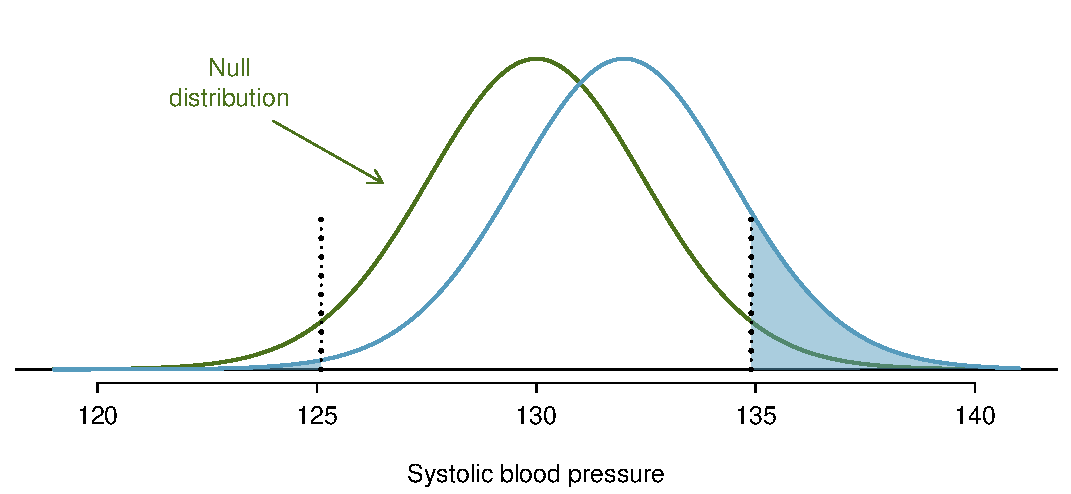
\includegraphics[width=\textwidth]{ch_inference_foundations_oi_biostat/figures/power132And141/power132And141}
\caption{The sampling distribution of $\bar{x}$ under two scenarios. Left: $N(130, 2.5)$. Right: $N(132, 2.5)$, and the shaded areas in this distribution represent the power of the test.}
\label{power132And141}
\end{figure}

The probability of rejecting the null hypothesis is called the \term{power}. The power varies depending on what we suppose the truth might be. In Example~\ref{computePowerIfMuIs132AndMu0Is130}, the difference between the null value and the supposed true mean was relatively small, so the power was also small: only 0.126. However, when the truth is far from the null value, where we use the standard error as a measure of what is far, the power tends to increase.

\begin{exercise}
Suppose the true sampling distribution of $\bar{x}$ is centered at 140. That is, $\bar{x}$ comes from $N(140, 2.5)$. What would the power be under this scenario? It may be helpful to draw $N(140, 2.5)$ and shade the area representing power on Figure~\ref{power132And141}; use the same cutoff values identified in Example~\ref{computePowerIfMuIs132AndMu0Is130}.\footnote{Draw the distribution $N(140, 2.5)$, then find the area below 125.1 (about zero area) and above 134.9 (about 0.979). If the true mean is 140, the power is about 0.979.}
\end{exercise}

\begin{exercise}
If the power of a test is 0.979 for a particular mean, what is the Type 2 Error rate for this mean?\footnote{The Type 2 Error rate represents the probability of failing to reject the null hypothesis. Since the power is the probability we do reject, the Type 2 Error rate will be $1-0.979 = 0.021$.}
\end{exercise}

\begin{exercise}
Provide an intuitive explanation for why we are more likely to reject $H_0$ when the true mean is further from the null value.\footnote{Answers may vary a little. When the truth is far from the null value, the point estimate also tends to be far from the null value, making it easier to detect the difference and reject $H_0$.}
\end{exercise}

\subsection{Statistical significance versus practical significance}

When the sample size becomes larger, point estimates become more precise and any real differences in the mean and null value become easier to detect and recognize. Even a very small difference would likely be detected if we took a large enough sample. Sometimes researchers will take such large samples that even the slightest difference is detected. While we still say that difference is \term{statistically significant}, it might not be \term{practically significant}.

Statistically significant differences are sometimes so minor that they are not practically relevant. This is especially important to research: if we conduct a study, we want to focus on finding a meaningful result. We don't want to spend lots of money finding results that hold no practical and applicable value.

The role of a statistician in conducting a study often includes planning the size of the study and determining the value of $\alpha$. Statisticians might first consult experts or scientific literature to learn what would be the smallest meaningful difference from the null value. They also would obtain some reasonable estimate for the standard deviation. With these important pieces of information, a sufficiently large sample size would be chosen so that the power for the meaningful difference is perhaps 80\% or 90\%. While larger sample sizes may still be used, statisticians in practice might advise against using them in some cases, especially in sensitive areas of research. While we note the statistical rigor in our hypothesis testing, we must also note that many of these tests must also stand up to practical significance in the real world.









%%%%%%%%%%%%%%HERE IS THE COMMENT%%%%%%%%%%%%%%%%%%%%%%%%%%%%
%%%%%%%%%%%%%%HERE IS THE COMMENT%%%%%%%%%%%%%%%%%%%%%%%%%%%%
%%%%%%%%%%%%%%HERE IS THE COMMENT%%%%%%%%%%%%%%%%%%%%
%%%%%%%%%%%%%%HERE IS THE COMMENT%%%%%%%%%%%%%%%%%%%%%%%%%%%%
-----------------------------------------------------------------------------------------------------------------------------------------------------
\begin{comment}
Statistical inference is concerned primarily with understanding the quality of parameter estimates. For example, a classic inferential question is, ``How sure are we that the estimated mean, $\bar{x}$, is near the true population mean, $\mu$?'' While the equations and details change depending on the setting, the foundations for inference are the same throughout all of statistics. We introduce these common themes in Sections~\ref{variabilityInEstimates}-\ref{cltSection} by discussing inference about the population mean, $\mu$, and set the stage for other parameters and scenarios in Section~\ref{aFrameworkForInference}. Some advanced considerations are discussed in Section~\ref{sampleSizeAndPower}. Understanding this chapter will make the rest of this book, and indeed the rest of statistics, seem much more familiar.

%%%%%%%%%%%%%%HERE IS THE COMMENT%%%%%%%%%%%%%%%%%%%%%%%%%%%%
\end{comment} %%%%%%%%%%%%%%HERE IS THE COMMENT%%%%%%%%%%%%%%%%%%%%
%%%%%%%%%%%%%%HERE IS THE COMMENT%%%%%%%%%%%%%%%%%%%%%%%%%%%%




%%%%%%%%%%%%%%FUTURE POTENTIAL EXAMPLESSS%%%%%%%%%%%%%%%%%%%%%%%%%%%%

\begin{comment}

\begin{exercise} \label{ebayAmazonOneSidedTestExercise}
\index{data!mario\_kart|(}
Ebay might be interested in showing that buyers on its site tend to pay less than they would for the corresponding new item on Amazon. We'll research this topic for one particular product: a video game called \emph{Mario Kart} for the Nintendo Wii. During early October 2009, Amazon sold this game for \$46.99. Set up an appropriate (one-sided!) hypothesis test to check the claim that Ebay buyers pay less during auctions at this same time.\footnote{The skeptic would say the average is the same on Ebay, and we are interested in showing the average price is lower.
\begin{itemize}
\setlength{\itemsep}{0mm}
\item[$H_0$:] The average auction price on Ebay is equal to (or more than) the price on Amazon. We write only the equality in the statistical notation: $\mu_{ebay} = 46.99$.
\item[$H_A$:] The average price on Ebay is less than the price on Amazon, $\mu_{ebay} < 46.99$.
\end{itemize}}
\end{exercise}


\begin{exercise} \label
{exerciseFor52EbayAuctionsToExamineMarioKartLessExpensiveThanAmazonConditions}
During early October, 2009, 52 Ebay auctions were recorded for \emph{Mario Kart}.\footnote{These data were collected by OpenIntro staff.} The total prices for the auctions are presented using a histogram in Figure~\ref{ebayMarioKartAuctionPriceHistogramFor3ConditionsExercise}, and we may like to apply the normal model to the sample mean. Check the three conditions required for applying the normal model: (1)~independence, (2)~at~least 30 observations, and (3)~the data are not strongly skewed.\footnote{(1) The independence condition is unclear. \emph{We will make the assumption that the observations are independent, which we should report with any final results.} (2) The sample size is sufficiently large: $n =52 \geq 30$. (3) The data distribution is not strongly skewed; it is approximately symmetric.}
\end{exercise}

\begin{figure}
   \centering
   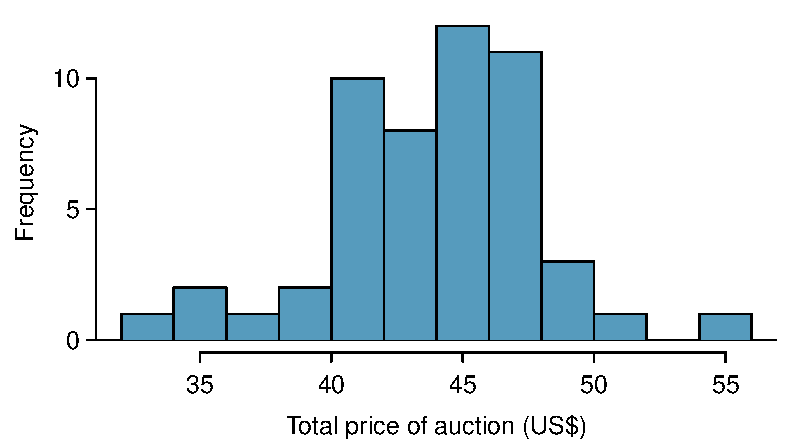
\includegraphics[width=0.68\textwidth]{ch_inference_foundations_oi_biostat/figures/ebayMarioKartAuctionPriceHistogramFor3ConditionsExercise/ebayMarioKartAuctionPriceHistogramFor3ConditionsExercise}
   \caption{A histogram of the total auction prices for 52 Ebay auctions.}
   \label{ebayMarioKartAuctionPriceHistogramFor3ConditionsExercise}
\end{figure}

\begin{example}{The average sale price of the 52 Ebay auctions for \emph{Wii Mario Kart} was \$44.17 with a standard deviation of \$4.15. Does this provide sufficient evidence to reject the null hypothesis in Exercise~\ref{ebayAmazonOneSidedTestExercise}? Use a significance level of $\alpha = 0.01$.}
The hypotheses were set up and the conditions were checked in Exercises~\ref{ebayAmazonOneSidedTestExercise} and~\ref{exerciseFor52EbayAuctionsToExamineMarioKartLessExpensiveThanAmazonConditions}. The next step is to find the standard error of the sample mean and produce a sketch to help find the p-value.
\begin{eqnarray*}
SE_{\bar{x}} = s/\sqrt{n} = 4.15/\sqrt{52} = 0.5755
\end{eqnarray*}
\begin{center}
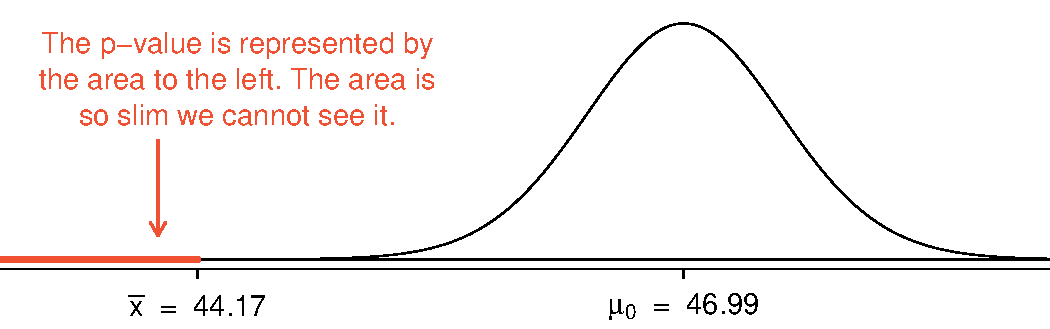
\includegraphics[height=35mm]{ch_inference_foundations_oi_biostat/figures/pVForEbayAmazonComparison/pVForEbayAmazonComparison}
\end{center}
Because the alternative hypothesis says we are looking for a smaller mean, we shade the lower tail. We find this shaded area by using the Z score and normal probability table: $Z = \frac{44.17 - 46.99}{0.5755} = -4.90$, which has area less than 0.0002. The area is so small we cannot really see it on the picture. This lower tail area corresponds to the p-value.

Because the p-value is so small -- specifically, smaller than $\alpha = 0.01$ -- this provides sufficiently strong evidence to reject the null hypothesis in favor of the alternative. The data provide statistically significant evidence that the average price on Ebay is lower than Amazon's asking price.
\index{data!mario\_kart|)}
\end{example}

\end{comment}


%%%%%%%%%%%%%%FUTURE POTENTIAL EXAMPLESSS END%%%%%%%%%%%%%%%%%%%%%%%%%%%%




%%%%%%%%%%%%%%%



















